%%%%%%%%%%%%%%%%%%%%%%%%%%%%%%%%%%%%%%%%%%%%%%%%%%%%%%%%%%%%%%%%%%%%%
%% This is a (brief) model paper using the achemso class
%% The document class accepts keyval options, which should include
%% the target journal and optionally the manuscript type. 
%%%%%%%%%%%%%%%%%%%%%%%%%%%%%%%%%%%%%%%%%%%%%%%%%%%%%%%%%%%%%%%%%%%%%
\documentclass[journal=jcisd8,manuscript=article]{achemso}

%%%%%%%%%%%%%%%%%%%%%%%%%%%%%%%%%%%%%%%%%%%%%%%%%%%%%%%%%%%%%%%%%%%%%
%% Place any additional packages needed here.  Only include packages
%% which are essential, to avoid problems later. Do NOT use any
%% packages which require e-TeX (for example etoolbox): the e-TeX
%% extensions are not currently available on the ACS conversion
%% servers.
%%%%%%%%%%%%%%%%%%%%%%%%%%%%%%%%%%%%%%%%%%%%%%%%%%%%%%%%%%%%%%%%%%%%%
\usepackage[version=3]{mhchem} % Formula subscripts using \ce{}
\usepackage{graphicx}
\usepackage{subcaption}

%%%%%%%%%%%%%%%%%%%%%%%%%%%%%%%%%%%%%%%%%%%%%%%%%%%%%%%%%%%%%%%%%%%%%
%% If issues arise when submitting your manuscript, you may want to
%% un-comment the next line.  This provides information on the
%% version of every file you have used.
%%%%%%%%%%%%%%%%%%%%%%%%%%%%%%%%%%%%%%%%%%%%%%%%%%%%%%%%%%%%%%%%%%%%%
%%\listfiles

%%%%%%%%%%%%%%%%%%%%%%%%%%%%%%%%%%%%%%%%%%%%%%%%%%%%%%%%%%%%%%%%%%%%%
%% Place any additional macros here.  Please use \newcommand* where
%% possible, and avoid layout-changing macros (which are not used
%% when typesetting).
%%%%%%%%%%%%%%%%%%%%%%%%%%%%%%%%%%%%%%%%%%%%%%%%%%%%%%%%%%%%%%%%%%%%%
\newcommand*\mycommand[1]{\texttt{\emph{#1}}}

\author{Andrew McNutt}
\author{Paul Francoeur}
\affiliation[University of Pittsburgh]
{Department of Computational and Systems Biology, University of Pittsburgh, Pittsburgh, PA}
\author{Rishal Aggarwal}
\affiliation[International Institute of Information Technology Hyderabad]
{Center for Computational Natural Sciences and Bioinformatics, International Institute of Information Technology, Hyderabad 500 032, India}
\author{Tomohide Masuda}
\affiliation[University of Pittsburgh]
{Department of Computational and Systems Biology, University of Pittsburgh, Pittsburgh, PA}
\author{Rocco Meli}
\affiliation[Oxford]{Oxford}
\author{Matthew Ragoza}
\author{Jocelyn Sunseri}
\author{David Ryan Koes}
\email{dkoes@pitt.edu}
\affiliation[University of Pittsburgh]
{Department of Computational and Systems Biology, University of Pittsburgh, Pittsburgh, PA}


%%%%%%%%%%%%%%%%%%%%%%%%%%%%%%%%%%%%%%%%%%%%%%%%%%%%%%%%%%%%%%%%%%%%%
%% The document title should be given as usual. Some journals require
%% a running title from the author: this should be supplied as an
%% optional argument to \title.
%%%%%%%%%%%%%%%%%%%%%%%%%%%%%%%%%%%%%%%%%%%%%%%%%%%%%%%%%%%%%%%%%%%%%
\title[GNINA 1.0]
  {GNINA 1.0: Molecular docking with deep learning}

%%%%%%%%%%%%%%%%%%%%%%%%%%%%%%%%%%%%%%%%%%%%%%%%%%%%%%%%%%%%%%%%%%%%%
%% Some journals require a list of abbreviations or keywords to be
%% supplied. These should be set up here, and will be printed after
%% the title and author information, if needed.
%%%%%%%%%%%%%%%%%%%%%%%%%%%%%%%%%%%%%%%%%%%%%%%%%%%%%%%%%%%%%%%%%%%%%
\keywords{molecular docking, deep learning, structure-based drug design}

%%%%%%%%%%%%%%%%%%%%%%%%%%%%%%%%%%%%%%%%%%%%%%%%%%%%%%%%%%%%%%%%%%%%%
%% The manuscript does not need to include \maketitle, which is
%% executed automatically.
%%%%%%%%%%%%%%%%%%%%%%%%%%%%%%%%%%%%%%%%%%%%%%%%%%%%%%%%%%%%%%%%%%%%%
\begin{document}

%%%%%%%%%%%%%%%%%%%%%%%%%%%%%%%%%%%%%%%%%%%%%%%%%%%%%%%%%%%%%%%%%%%%%
%% The "tocentry" environment can be used to create an entry for the
%% graphical table of contents. It is given here as some journals
%% require that it is printed as part of the abstract page. It will
%% be automatically moved as appropriate.
%%%%%%%%%%%%%%%%%%%%%%%%%%%%%%%%%%%%%%%%%%%%%%%%%%%%%%%%%%%%%%%%%%%%%
\begin{tocentry}

\end{tocentry}

%%%%%%%%%%%%%%%%%%%%%%%%%%%%%%%%%%%%%%%%%%%%%%%%%%%%%%%%%%%%%%%%%%%%%
%% The abstract environment will automatically gobble the contents
%% if an abstract is not used by the target journal.
%%%%%%%%%%%%%%%%%%%%%%%%%%%%%%%%%%%%%%%%%%%%%%%%%%%%%%%%%%%%%%%%%%%%%
\begin{abstract}

\end{abstract}

\paragraph{Authorship}  I want everyone who has contributed meaningfully to gnina to be included in this paper, but am anticipating that Paul and Drew will do most of the analysis with feedback from everyone else.\

\paragraph{Journal} Most likely JCIM, but if the results are impressive might take a stab at Nature Methods (which would involve a lot of refactoring to shove things into the supplement).

%%%%%%%%%%%%%%%%%%%%%%%%%%%%%%%%%%%%%%%%%%%%%%%%%%%%%%%%%%%%%%%%%%%%%
%% Start the main part of the manuscript here.
%%%%%%%%%%%%%%%%%%%%%%%%%%%%%%%%%%%%%%%%%%%%%%%%%%%%%%%%%%%%%%%%%%%%%
\section{Introduction}

Molecular docking is a computational procedure in which the non-covalent bonding of macromolecules is predicted, most often a protein and a ligand. The goal of this prediction is the binding affinity and conformation of the small molecule in its minimal energy state. Docking is composed of two main steps, sampling and scoring. Sampling refers to an extensive search of the conformational space of the docking molecule. Proper sampling requires thorough coverage of the conformational landscape of both the ligand and the protein. The flexibility of the ligand and the protein determine the conformations that can be accessed, expanding the search space when flexibility of either molecule is increased. The other vital piece of a molecular docking software is the scoring function. Every pose that is sampled by the algorithm must be evaluated for its fitness in comparison to other conformations. The scoring function determines the conformations that are retained from the sampling of the search space and ranks the retained poses in order of their likelihood of being correct. The final output is a set of ranked poses of the docked molecule that are then given a binding affinity for the larger macromolecule. Determination of the correct binding pose of the small molecule allows us to properly determine the binding affinity of the molecule and affords the opportunity to utilize the pose for lead optimization of the small molecule. Correct evaluation of binding affinity is critical for downstream tasks such as virtual screening or for determining if a compound is important for more experimental analysis. Molecular docking must provide a pose and a binding affinity quickly for its use in the drug discovery pipeline. Sampling the entire conformational space of a molecule is not a quick task, therefore, we must compromise on the speed and accuracy of the docking to provide poses that are close to native while not requiring the full search of the conformational space. The compromise requires our docking software to focus on the accuracy and ranking power of the scoring function to pull out the best conformations early on in sampling.

Scoring functions provide a mapping from the conformational space of the two molecules to the real number line so that poses may be ranked. Typically, scoring functions are put into two categories; empirical and knowledge based. Knowledge based scoring functions leverage the statistics from a set of structural binding data. A number of properties are computed from structures of protein-ligand complexes, such as atom-atom pairwise contacts. The calculated frequencies can be used in a method such as Potential Mean Force, which creates a potential based on the boltzmann distribution of the properties, to calculate the score of a pose. Knowledge based scoring functions tend to generalize well and calculations of scores are quick at test time. However, they require a large database of known structures, largeley ignore the effect of solvents, and can be difficult to intepret when trying to understand a score. Empirical scoring functions build on knowledge based functions by combining the knowledge from known structures with force field terms. The force field terms include non-covalently bonded terms like ..., these are often weighted with tuned hyperparameters. A large proportion of docking software use empirical scoring functions, including ... \cite{}. Unlike knowledge based scoring functions, empirical scoring functions allow simple interpretation of what is contributing to the score. They are less prone to overfitting than scoring functions only including force-field terms, but the combination of terms creates a difficulty for determining where errors come from. Both of these categories of scoring functions are limited to features extracted from structural information and assume there is a linear relationship between the features and the binding affinity. The scoring function utilized in Autodock Vina (called `Vina') is an empirical scoring function explicitly tuned to structural data\cite{trott2010autodock}. The scoring function is a weighted sum of functions scoring the interactions of atoms based on their distance. The functions include gaussian terms, repulsion, hydrophobic, hydrogen bonding, and the number of rotatable bonds. The weights of the terms beind denoted by a non-linear fit to structural data. A mathematically tractable scoring function is essential as the sampling strategy employed, Iterated Local Search global optimizer, utilizes the gradients of each term within the scoring function to update the ligand conformation, thereby ensuring that the local minimum is reached. The success of Vina, an empirical scoring function with a non-linear fit to the data, we must look for alternative methods that are able to model non-linear relationships and extract features directly from structural information without explicit featurization.

Machine learning(ML) algorithms learn arbitrary relationships between observations and outputs. There has been considerable progress in other biomedical fields with the utilization of ML models, including drug-design and medical image classification [need citations]. However, they require a large amount of data to properly generalize to unseen information. The last 20 years has seen a noteworthy increase in the quanity of available structures with experimentally annotated binding data\cite{}. A plethora of sites host a range of annotated structural information, including PDBBind and BindingDB [need citations]. This information has been utilized to leverage machine learning algorithms as scoring functions. A number of traditional ML approaches have been used as scoring functions, including random forests (RF-Score and SFCScore), support vector machines (SVR-SF, ID-Score, SVR-EP), artificial neural networks (NNscore and BsN-Score), and gradient boosted decision trees (BT-dock and ESPH T-Bind)\cite{liu2017forging,zilian2013sfcscore,li2011svr,li2013idscore,durrant2010nnscore,ashtawy2015bsn,btdock,cang2018integration}. These ML methods have been able to match or exceed existing traditional scoring functions. ML methods allow a more robust fit to the training data, but are limited to the features explicitly extracted from structural data.

Deep Learning(DL) methods allow direct inference of features from inputs. These methods have demonstrated success in a variety of fields, such as computer vision and natural language processing\cite{krizhevsky2017imagenet,brown2020language}. In recent years, there has been significant progress with DL methods in the drug discovery field with many models emplying a convolutional framework. Convolutional Neural Networks(CNN) leverage convolutions to infer features directly from input tensors, usually images. CNNs have shown potential in virtual screening (AtomNet, DeepVS, \cite{Ragoza2017}) and binding affinity prediction (PotentialNet, $K_{DEEP}$, Pafnucy)\cite{wallach2015atomnet,jimenez2018k,pereira2016boosting,feinberg2018potentialnet,stepniewska2018development}. A number of methods have been proposed to capitalize on the power of DL scoring functions. MedusaNet uses a CNN within the docking pipeline to guide the sampling of the base sampling method\cite{jiang2020guiding}. The base docking method, Medusa, provides a variety of ligand poses that are translated to a 3D coordinate representation which the CNN evaluates for determination of whether to keep the pose. Nguyen et. al. \cite{nguyen2020mathdl} describe a generative adversarial network(GAN) for pose prediction. Their network utilizes an encoder with low-dimensional mathematical representations of the protein-ligand complex and a decoder utilizing convolutional layers to generate and rank ligand poses for the D3R grand challenge. Masuda et. al. \cite{masuda2020generating} use a receptor structure as the prior to their GAN to simultaneously sample and score novel molecular targets.

\textit{preview what is to come}

\section{Methods}

\subsection{Molecular Docking Pipeline}
Gnina is a fork of Smina which is a fork of Autodock Vina. The docking pipeline of gnina utilizes the enhanced support for scoring enabled in Smina to allow the use of CNNs as scoring functions. In typical usage, Gnina is provided with a receptor structure, a ligand structure, and the coordinates for a binding pocket on the receptor. Open Babel\cite{o2011open,babelopen}, a chemical toolbox allowing the reading and writing of over 100 chemical file formats, is used for parsing the inputs, allowing many of the commonly used structural data formats (i.e. PDB, sdf, mol, etc.). The binding pocket or autobox is then setup using the minimum and maximum values for the x, y and z coordinates of the input for the binding pocket to define a rectangular prism. An additional spacing is added to the autobox, termed autobox add, on all sides of the box defining the binding pocket. Then the ligand is parsed with Open Babel. If any side of the box is smaller than the longest distance between any two atoms in the ligand, then those sides are extended to that longest distance, ensuring that the ligand can rotate freely within the defined binding box.

Next the scoring functions are setup to perform the coarse grained calculations during the sampling and the high resolution evaluations for the refinement and affinity measurement. Similar to smina, the user can input their own scoring function to gnina or use one of the built-in scoring functions, i.e. Vina, vinardo, etc. The scoring function is then used to precalculate a grid of pseudo energy to guide the sampling process. The scoring function is calculated for all of the atom types specified in the input ligand, on a grid defined by the binding box. The scoring function is determined exactly for each point on the grid with values between grid points calculated with a linear interpolation. CNN models are loaded, if one of the CNN scoring options are chosen, from the built in CNN models or from a user specified weights and/or model file. The available built-in CNN models include Crossdock\_Default2018, Dense, General\_Default2018, Redock\_Default2018, and Default2017. Each of these CNN models, excluding Default2017, has five variants which are trained on the same data and have the same architecture but are initialized with a different random seed. The architecture and training of these models are described in \cite{francoeur2020three,Ragoza2017}. With all of the setup complete, the docking procedure begins.

The docking procedure is based on a monte carlo sampling method. The exhaustiveness defines the number of monte carlo chains that are run for the ligand, by default eight chains will be run. The number of steps for the monte carlo chains are calculated based on the number of mobile atoms and the number of degrees of freedom within the docking ligand. Each monte carlo chain randomly mutates the ligand by randomly selecting one of the following operations; random translation, random rotation of the entire molecule, and randomly setting the torsional angles of the ligand. The mutation favors the random resetting of the torsional angles over the other mutations. After the mutation, the ligand is minimized using the precalculated energy grid and the energy of the minimized conformation is calculated. The energy for this new minimized conformation determines if it will be accepted using the metropolis acceptance criterion. Each monte carlo chain retains a predefined number of ligand conformations, either the number of modes or the number of monte carlo saved whichever is greater.

Following the completion of the monte carlo sampling, the saved conformations from each monte carlo chain are added together into a list and the top scoring conformations are retained for further analysis. The number of top scoring conformations retained is again the number of modes or the number of monte carlo saved whichever is greater. The top scoring conformations are then refined using the high resolution scoring function to ensure the ligand is within the autobox. After the ligand pose has been refined, the final affinities are calculated for the pose using the specified CNN models and the specified scoring function. Finally the top scoring conformations are sorted based on one of the scores, determined by the user, and output with Open Babel in the user specified format.

The usage of the CNN models within the docking pipeline can be selected by the user. If "none" is selected for the CNN scoring option, then the CNN models are not used at all in the docking pipeline, making the pipeline identical to the smina pipeline. When "rescoring" is selected, the specified CNN models are not used until the final sorting of the refined ligand conformations. The specified CNN models are used to score each of the ligand conformations and the output ligand conformations are resorted based on the score calculated by the CNN model(s). The "refinement" option utilizes the CNN for the refinement of the ligand poses after they have been selected by the monte carlo chains and then sorts the refined ligand conformations by the CNN score for output. Finally, the "all" option utilizes the CNN for all aspects of the docking pipeline including the minimization within the monte carlo chains, the refinement after the monte carlo chains, and the sorting of the final output. 


\subsection{Data}
There are two primary ways to use a molecular docking platform, redocking a cognate ligand to its receptor and docking a ligand to a receptor that has no known binding pose. In order to best evaluate the performance of gnina for molecular docking we evaluate its performance on both of these tasks. Redocking the cognate ligand easily demonstrates the sampling and scoring power of the molecular docking pipeline, as the root mean square deviation (RMSD) from the crystal pose can be measured to determine the accuracy of the produced poses. Analysis of redocking requires a set of high quality structures in which the native binding pose of the ligand has been solved, for this purpose we utilize the PDBbind 2019 refined set. The PDBBind database is a currated set of protein ligand binding information containing both structural information and binding affinity. The PDBBind database is updated annually with new experimentally determined structures annotated with binding affinity data. The refined set is a subset of the entire PDBbind dataset that filters the structures with resolution higher than 2.5 A, high quality affinity measurements, and proper protein-ligand complexes. The 2019 release of the refined set contains 4,852 high quality crystal structures of native protein-ligand binding poses. However, redocking is not the normal use case of a molecular docking pipeline. Docking will ordinarily be performed on new systems of proteins and ligands that have no co-crystalized structure. Often a ligand will be docked to a crystal pose of a receptor in which the co-crystallized ligand was a different molecule. A recently published dataset provides a benchmark precisely for this task\cite{wierbowski2020cross}. The crossdocking dataset is composed of 95 unique protein targets with an average of 46 ligands per target. Additionally, this crossdocking dataset provides a meaningful method for the evaluation of the RMSD from the known and predicted poses. ProDy\cite{bakan2011prody} was used to separate the complexes into a separate protein and ligand file while removing any water or other extra crystallized molecules. Our goal is the binding pose prediction of small molecule targets, therefore we utilized RDKit\cite{rdkit} to filter both the redocking and crossdocking datasets to include only ligands with molecular masses greater than 150 kD and less than 1000 kD, any ligand that was not parsable with RDKit was also removed. The final sets were composed of 4,260 and (crossdocking set size) for the redocking and crossdocking datasets, respectively.

Still need to talk about subsampling of crossdocking data and the core set for benchmarks

\subsection{Smina Comparison}
Gnina is a fork of Smina that allows the utilization of CNN models as scoring functions. Therefore, without the use of the CNN models gnina should function exactly as Smina does. Unlike Smina, Gnina does computation of the scores\textbf{(is this true)?} with double precision rather than float precision due to the need to shift calculations to the GPU due to the efficiency of CNN calculations. Therefore, we must ensure that the use of this double precision does not negatively affect the docking power of the pipeline. The effect of this precision change can be evaluated by performing the same docking calculation with both softwares and comparing the results. We ran both Gnina and Smina on the redocking set using the same random seed and default values to ensure that the change of the floating point precision will not affect the results. 

\subsection{Optimal Model Selection}
The scoring function is vital to the performance of the molecular docking pipeline. Due to the high computational cost of applying the CNN models to the conformations selected by the smina scoring function, we must select a subset of the available models that provides accurate dockings while limiting computational cost. The default CNN model ensemble was selected using the forward algorithm. The ensemble was built in an iterative process using the "rescoring" option for CNN scoring so as to minimize the computational time for each iteration. In each round of the selection, models were chosen for their ability to score and rank a low RMSD conformation as the first pose. In each round we evaluate all of the versions of each CNN model(i.e. Dense, Dense\_1, Dense\_2, Dense\_3,Dense\_4). In the first round of selection, all of the CNN models were tested for their individual ability to predict low RMSD poses on both The Crossdock2020 and PDBbind dataset. The next round of selection required testing of all two model combinations with the model selected in the first step. Model selection continued, exploring all possible combinations of the built-in CNN models. The selection process was concluded after five CNN models were selected.

After the selection of the new default CNN model ensemble, we must evaluate the performance boost that this ensemble provides over any single CNN model or an ensemble of random initializations of the same CNN model type. We again compare the CNN model(s) performance on both the redocking and the crossdocking tasks. The CNN models are used in the "rescoring" option for the CNN scoring to output 10 ligand conformations. The RMSD to the known binding pose for each of the output conformations are computed with Open Babel's obrmsd function. If the pose is less than $2\,\AA$ then we consider the pose to be "good". The percentage of systems with a pose less than $2\,\AA$ is calculated for each dataset. We then compute the cumulative number of systems with a pose less than $2\,\AA$, so that at the second pose we are considering if either the first or second pose is less than $2\,\AA$ for a given system.

\subsection{Optimal Running Method}
Gnina allows the usage of the CNN models in various steps of the molecular docking process. The CNN scoring option allows the user to change how the CNN is used to evaluate a ligand pose. If the CNN is not used at all in the scoring process, "none" option, then the molecular docking pipeline is the same as Smina. The "rescoring" option is the lowest computational cost of the options that utilize the CNN models. The CNN models are used to score and resort the ligand conformations selected and refined by the non-CNN scoring function, usually the Vina scoring function. The next option in terms of computational cost is "refinement" which uses the CNN models for the refinement of the ligands after they have been selected by the monte carlo chains, which are still utilizing the non-CNN scoring function. In addition to refining the ligand conformations, the CNN models are used to score and resort the output poses, as the "rescore" option does. The "all" option uses the CNN models as the scoring function throughout the course of the molecular docking procedure. The CNN model is used for the selection process within the monte carlo chains, the refinement process after monte carlo selection, and the scoring and resorting of the poses before output. This option is very computationally intensive as the CNN must be constantly queried for the energy of a particular conformation during the monte carlo sampling procedure.

The default usage of the CNNs within the Gnina docking pipeline demands high accuracy while limiting computational and time cost. Therefore, each of the CNN scoring options must be evaluated both for performance and the time taken to perform. Performance of the docking procedure can be calculated on both the redocking and crossdocking datasets by determining the percentage of systems that have an RMSD less than 2 $\AA$ for each dataset. To this end, gnina is used with one of the CNN scoring options with the CNN ensemble selected above to compute 10 ligand poses for each protein ligand system. A RMSD is calculated from the known crystal pose, or known binding pose for crossdocking, using the Open Babel obrmsd function. We can then asses the number of systems that have an RMSD less than 2 $\AA$ from the known binding pose. Properly benchmarking the time for the various CNN scoring options on both the redocking and crossdocking datasets would take a significant amount of time, so we utilize the PDBbind Core Set to determine the time cost for each CNN scoring option. The docking time is calculated per system using the hyperfine benchmarking tool\cite{}, performing a minimum of 5 runs and calculating the average. The average docking time is then computed over the whole PDBbind Core set, to provide the average time for one docking run on an average protein-ligand system.

\subsection{Default Settings}
Gnina has many settings that alter the molecular docking pipeline. A default value must be found for each of these settings to ensure the user minimal tuning to their particular problem. In exploring the various values of the settings we must find the optimal value for both the redocking and the crossdocking datasets. Additionally, we must also consider that the user may not know the exact location of the binding pocket on the receptor and will likely have to use the entire protein as the autobox for the docking pipeline. Therefore, our setting exploration must consider the case in which the specific binding pocket is known and the case in which the whole protein is used to define a binding box. Some settings directly impact the sampling procedure, such as exhaustiveness, number of modes, number of monte carlo saved, and minimum RMSD filter. These settings control, to some extent, the extensiveness of the search during the monte carlo sampling procedure. As previously stated, the exhaustiveness determines the number of monte carlo chains run during the sampling procedure. Autobox add increases the size of the search space that the monte carlo chains are sampling, the box defined by the input autobox ligand is increased in size on all 6 sides by the value of autobox add. The number of modes determines the number of ligand poses output by gnina at the completion of the docking prodedure. This is separate from the number of monte carlo saved, which defines the number of  ligand poses saved for each monte carlo chain. The number of ligand poses retained after all of the monte carlo chains are completed is determined by either the number of modes or the number of monte carlo saved, whichever is larger. After all of the monte carlo chains have run and the runs are being combined, the minimum RMSD filter removes poses with a relative RMSD less than the value set for the filter so that the poses returned by the docking procedure are all different from one another. When using the CNN for scoring or refinement, another important setting is how many different rotations of the ligand conformation the CNN is able to see. The CNN models are ideally rotationally invariant as there are random roations of examples during training, the ability to see multiple rotations of the same conformation may make the CNN able to correctly calculate the score and energy.

Evaluations for all of the settings are carried out on both the redocking and crossdocking datasets. Each setting is varied individually using the optimal CNN model ensemble determined above. The exhaustiveness was explored in powers of two, due to the parallel computations of the monte carlo chains, going from four to 16. Exhaustiveness was explored again for the whole protein docking procedure, from eight to 64. The CNN rotations were explored for the values: 0, 1, 5, 10, and 20 (where 0 denotes a random rotation of the ligand conformation and 1 denotes a specific rotation of the ligand conformation). Values of 0.5, 1.0, and 1.5 were used to test the setting of minimum RMSD filter. The number of monte carlo saved was tested on multiples of 20, ranging from 20 to 100. The number of modes was evaluated using 9 and 100. Each value produced a set of poses, RMSD was determined for each output pose using Open Babel, and the percentage of systems with a RMSD less than 2 $\AA$ was calculated for each dataset.

\subsection{Gnina Performance Evaluation}

\section{Results}
\subsection{Smina Comparison}
Gnina was run without usage of CNN models in the molecular docking pipeline. Results for both redocking and crossdocking do not show a significant difference for the poses output from Gnina with no CNN and Smina (Supplement). A majority of the output poses are exactly the same, with slight differences seen for some output poses. The performance of Gnina with no CNN is slightly better than that of Smina using the same settings.

\subsection{Optimal Model Selection}
\begin{figure}
	\begin{subfigure}[b]{0.48\textwidth}
		\centering
		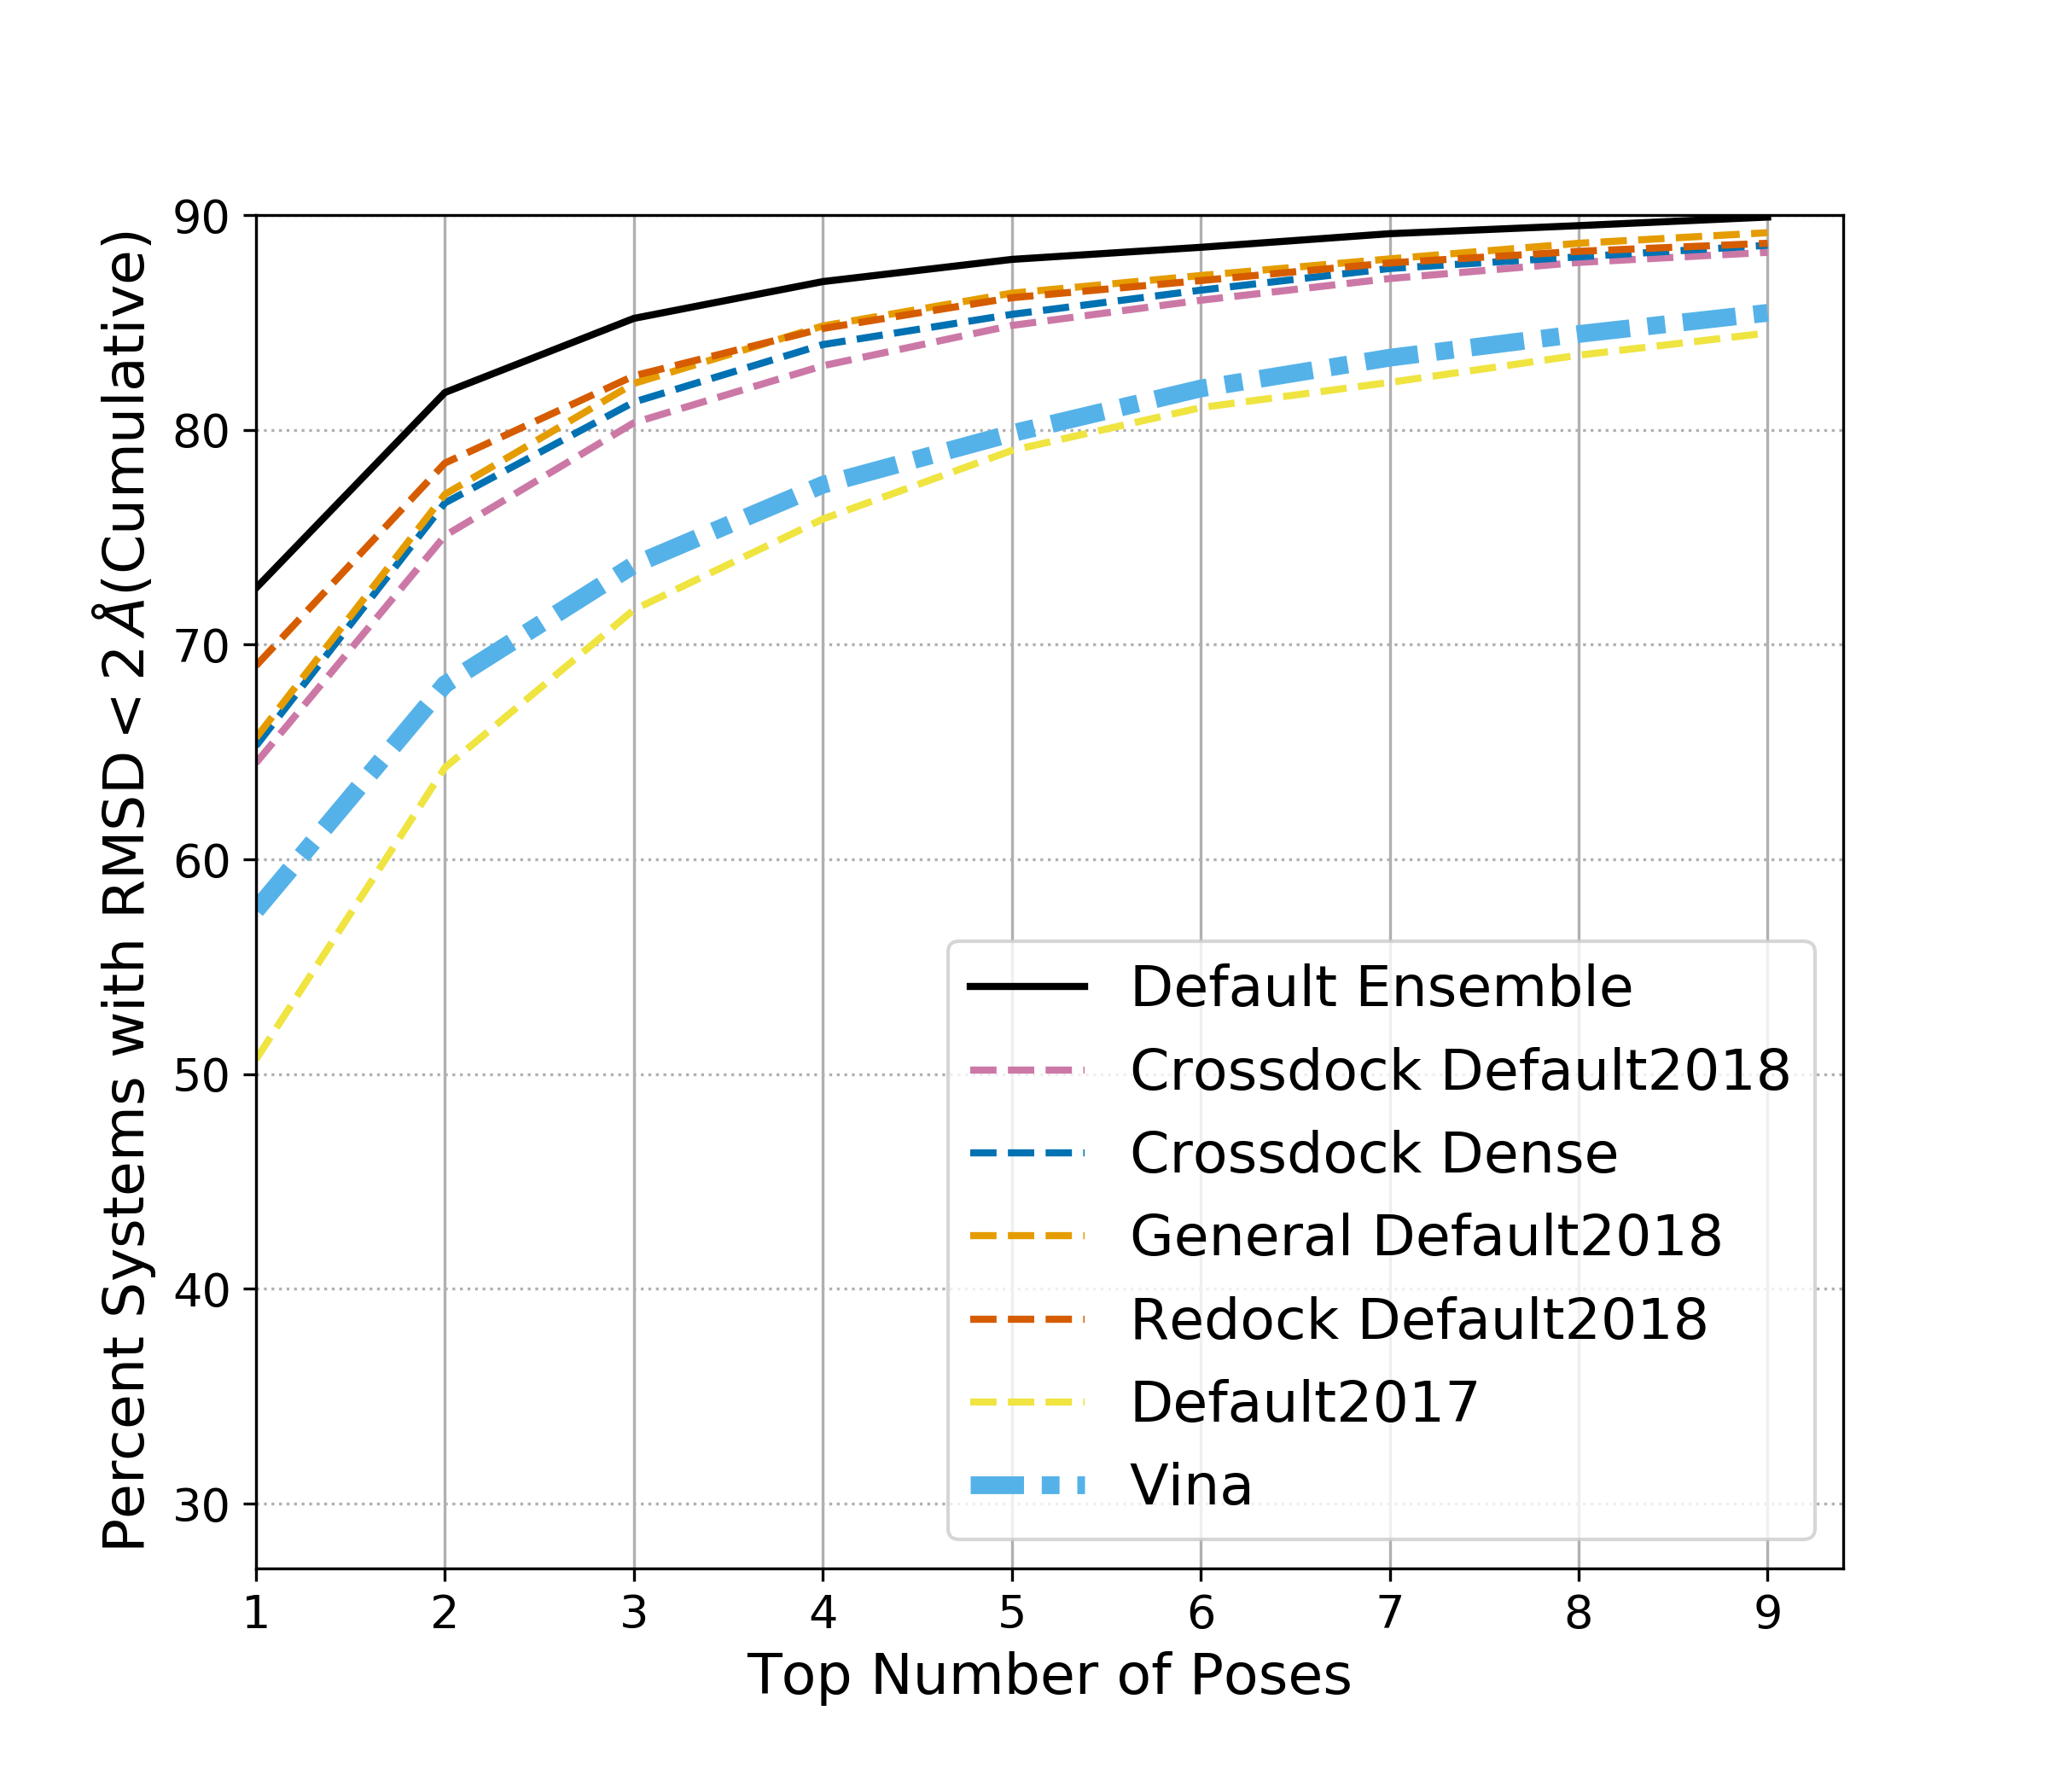
\includegraphics[width=\textwidth]{figures/redocking/rescore_single_models_line.png}
		\caption{Redocking}
		\label{fig:resc single rd}
        \end{subfigure}    
	\begin{subfigure}[b]{0.48\textwidth}    
		\centering
		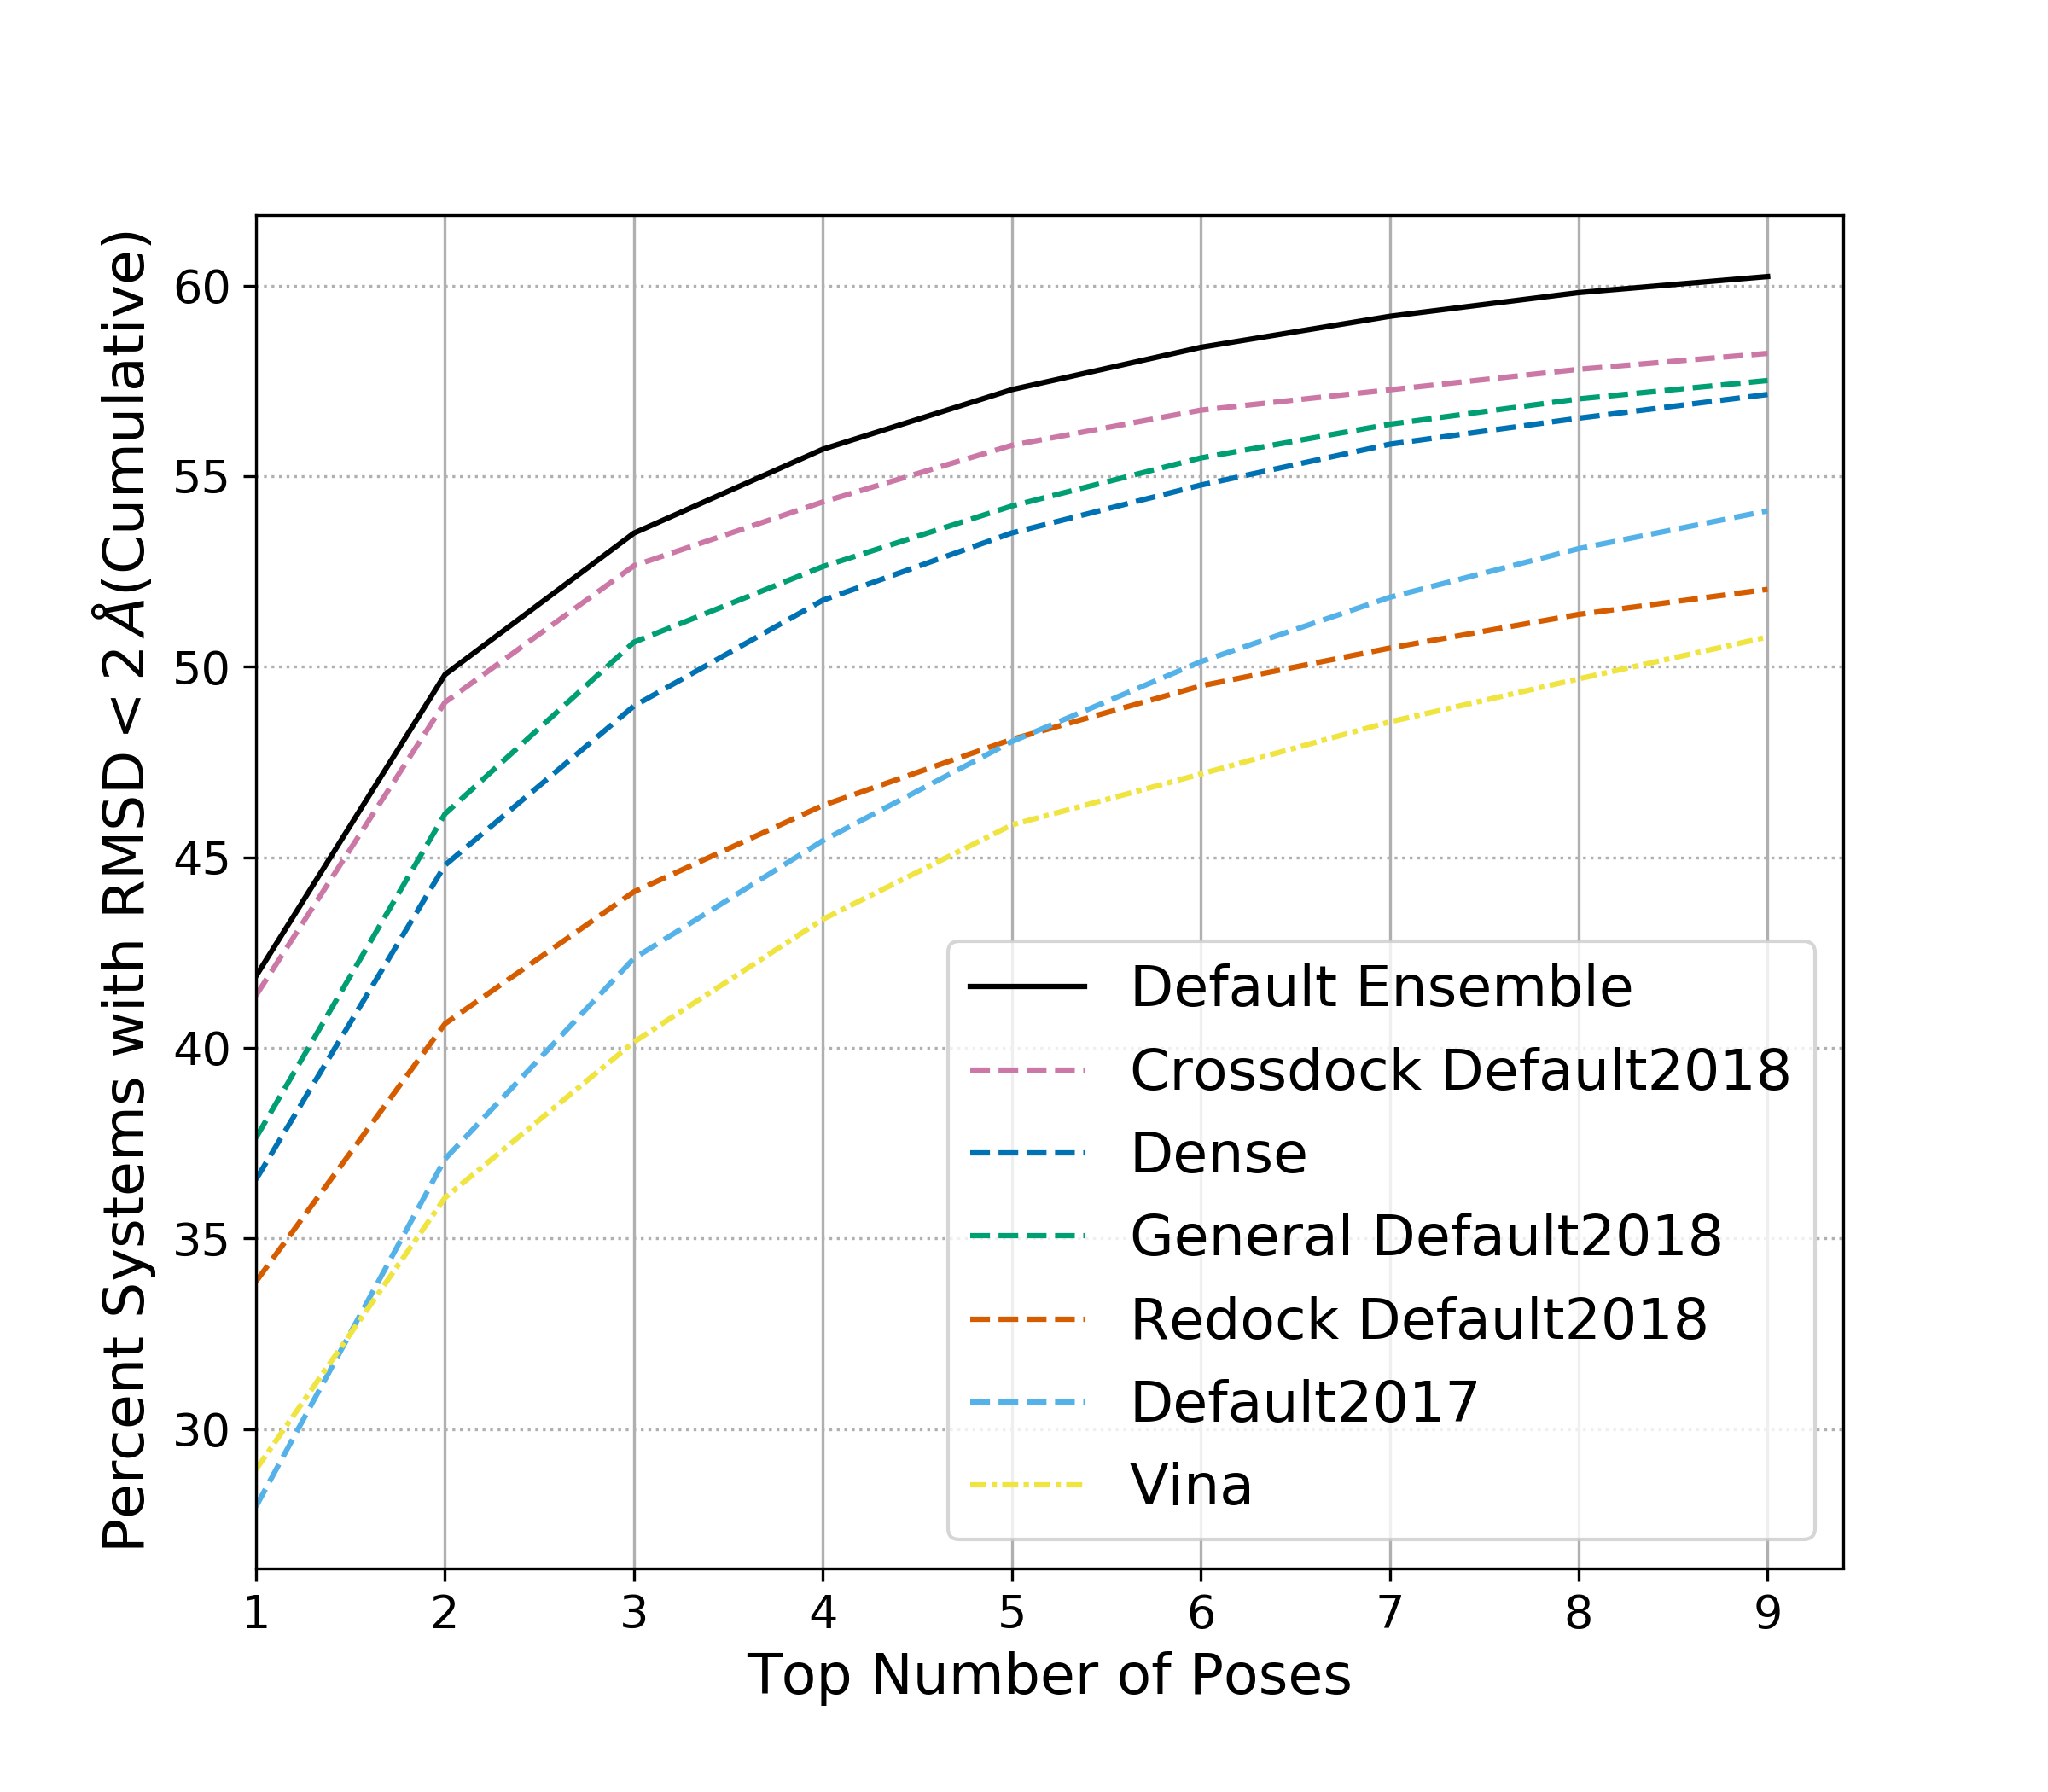
\includegraphics[width=\textwidth]{figures/crossdocking/rescore_single_models_line.png}
		\caption{Crossdocking}
		\label{fig:resc single cd}
        \end{subfigure}    
	\caption{Percentage of systems with RMSD to known binding pose less than $2\,\AA$ for each pose with results being cumulative}
	\label{fig:rescsingle}
\end{figure}    
The model selection procedure selected five models whose combined performance on ranking low RMSD poses first performance was optimal. The table for the model selection process can be seen in (supplemental table). The selected five selected models are Dense\_4, General\_Default2018\_3, Dense\_3, Crossdock\_Default2018, and Redock\_Default2018\_2. The performance of the model ensemble is compared to the single model options in \ref{fig:rescsingle}. We can see that the newly selected Default Ensemble significantly outperforms all of the single models on both the redocking task and the crossdocking task. All models are able to rank poses with low RMSD better than Vina. 


When the Default Ensemble is compared to the ensembles of each of the CNN model types, the ensembles consisting of each random intialization of the given CNN model type, we see that the Default Ensemble is able to outperform all of the ensembles composed of one model type\ref{fig:resc ens}. The diversity of models within the Default Ensembles allows better ranking of the poses due to the diversity of training data for each model type. The All Ensemble is the ensemble composed of all possible CNN models built-in to the Gnina software. The Default Ensemble is able to meet or exceed the performance of this large ensemble. The CNN models in the Default Ensemble are a subset of the models in the All Ensemble.

\begin{figure}
	\begin{subfigure}[b]{0.48\textwidth}
		\centering
		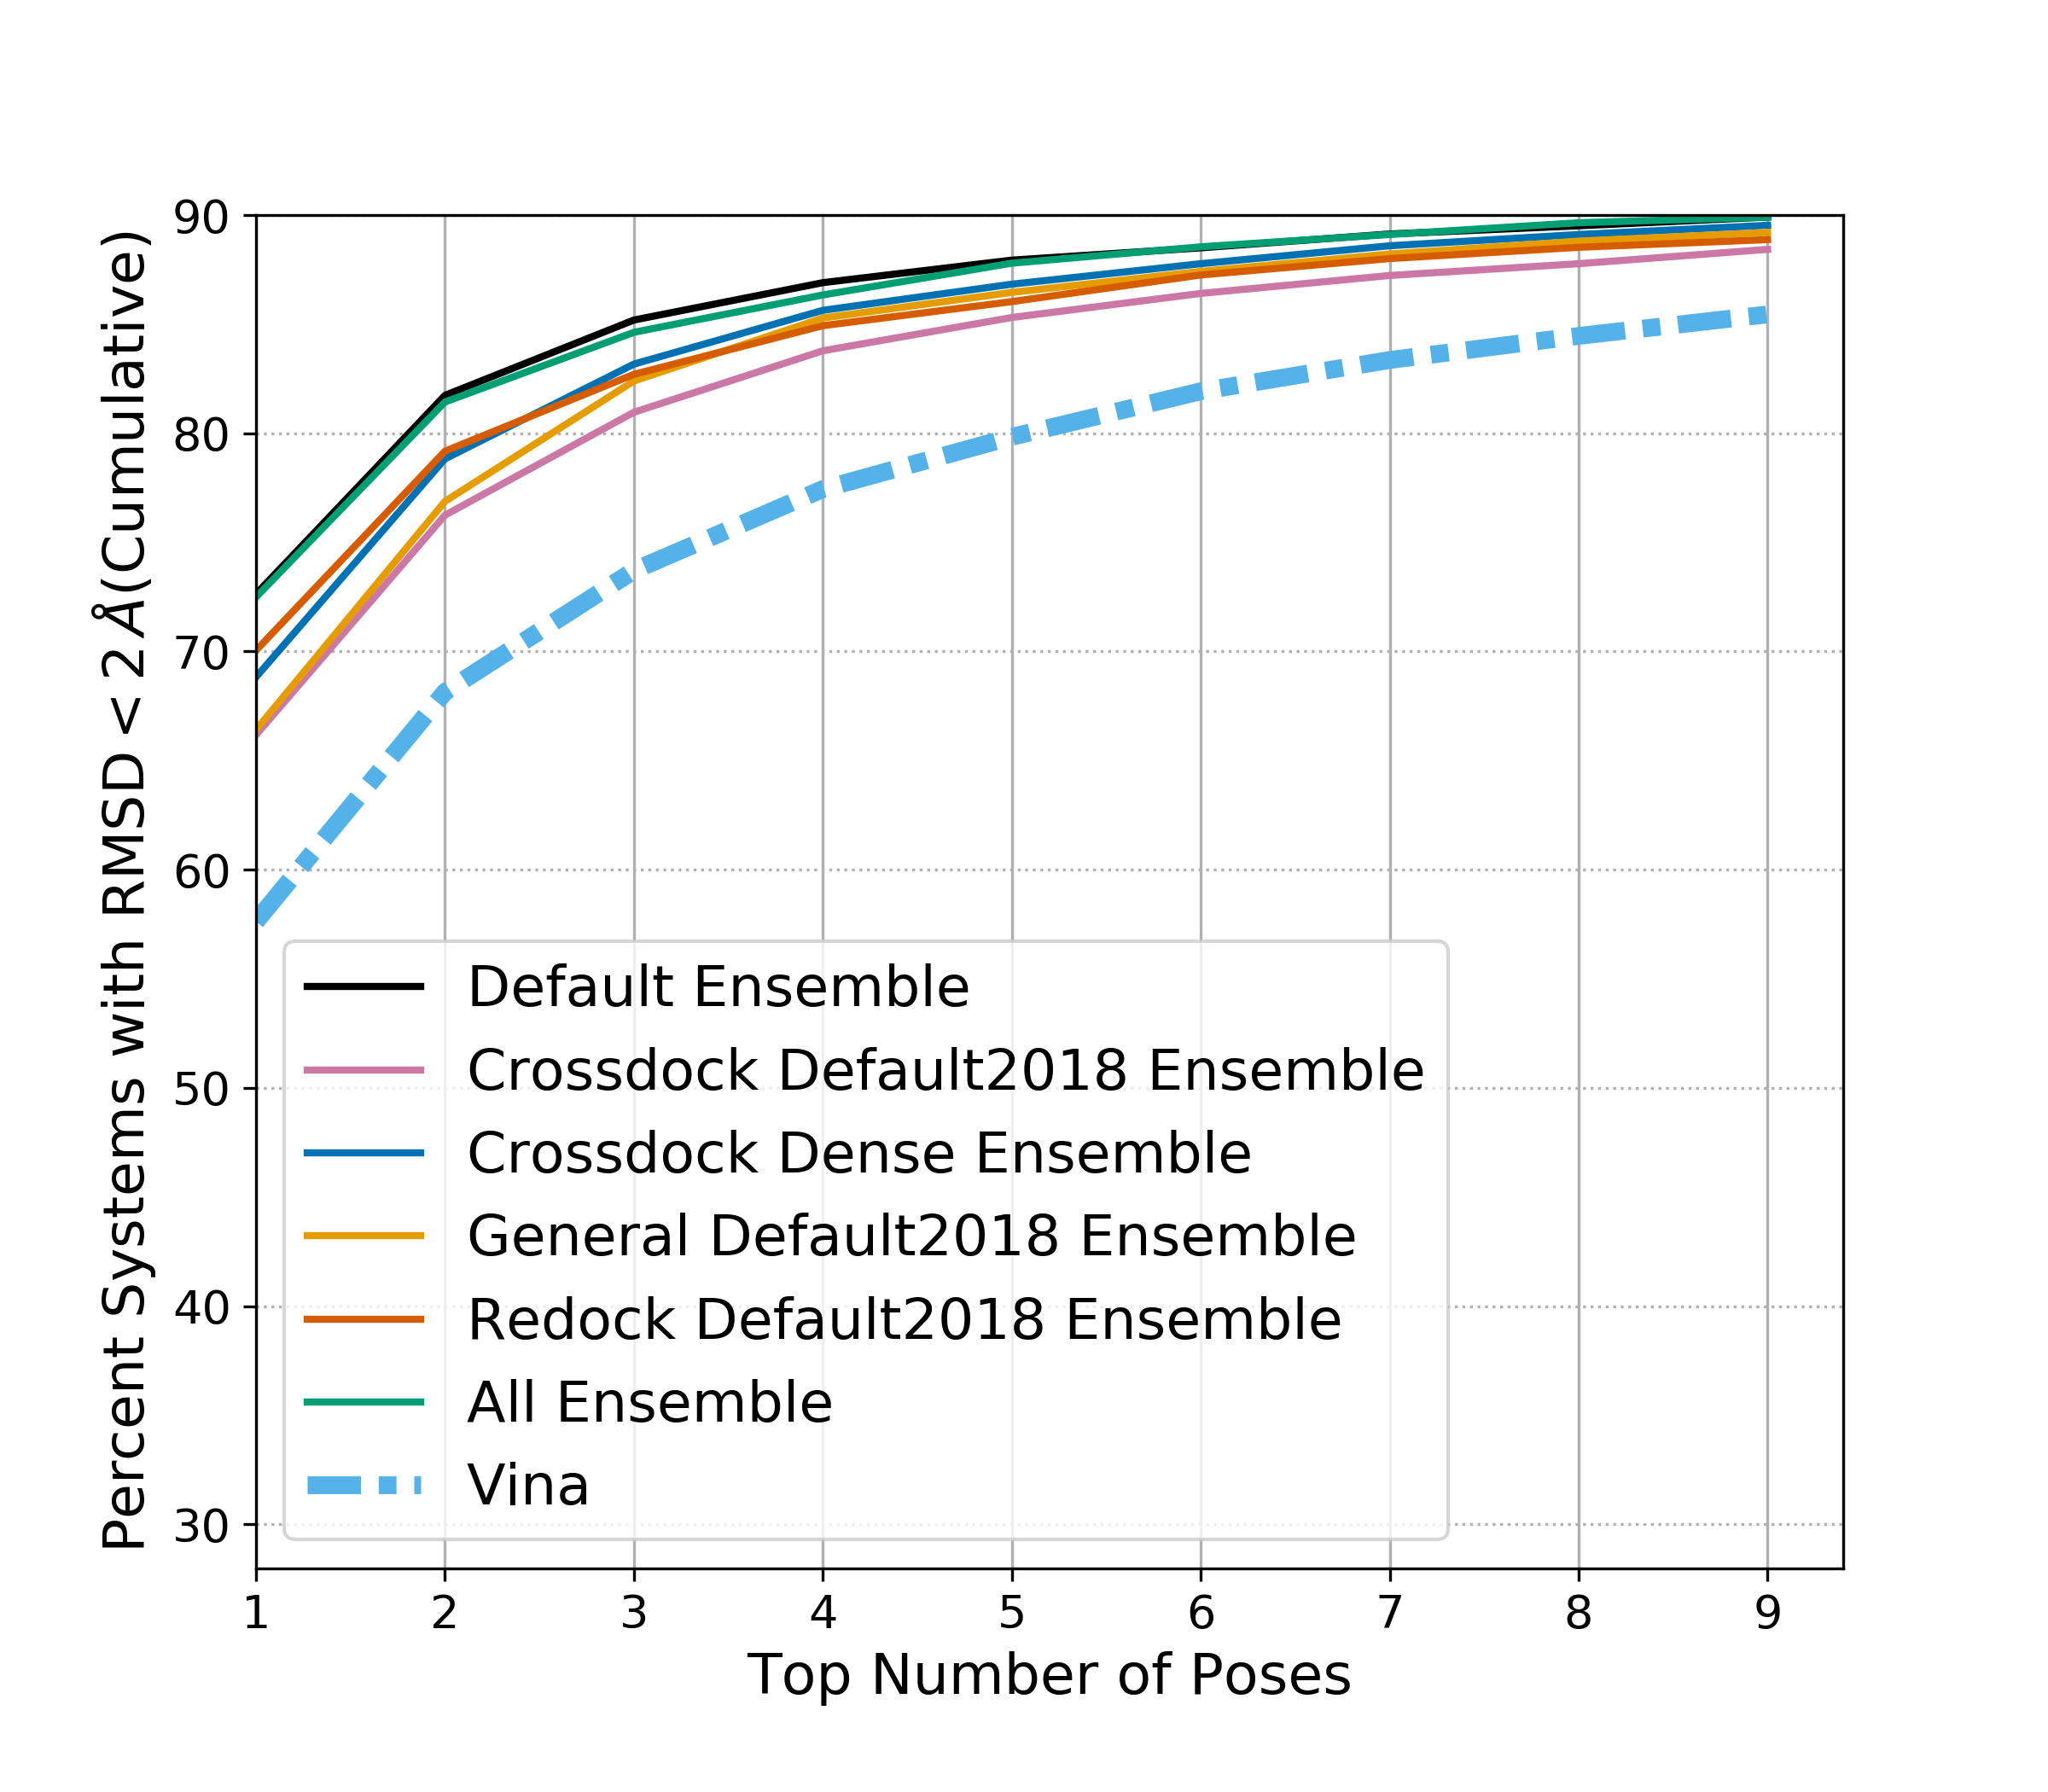
\includegraphics[width=\textwidth]{figures/redocking/rescore_ensembles_line.png}
		\caption{Redocking}
		\label{fig:resc ens rd}
        \end{subfigure}    
	\begin{subfigure}[b]{0.48\textwidth} 
		\centering
		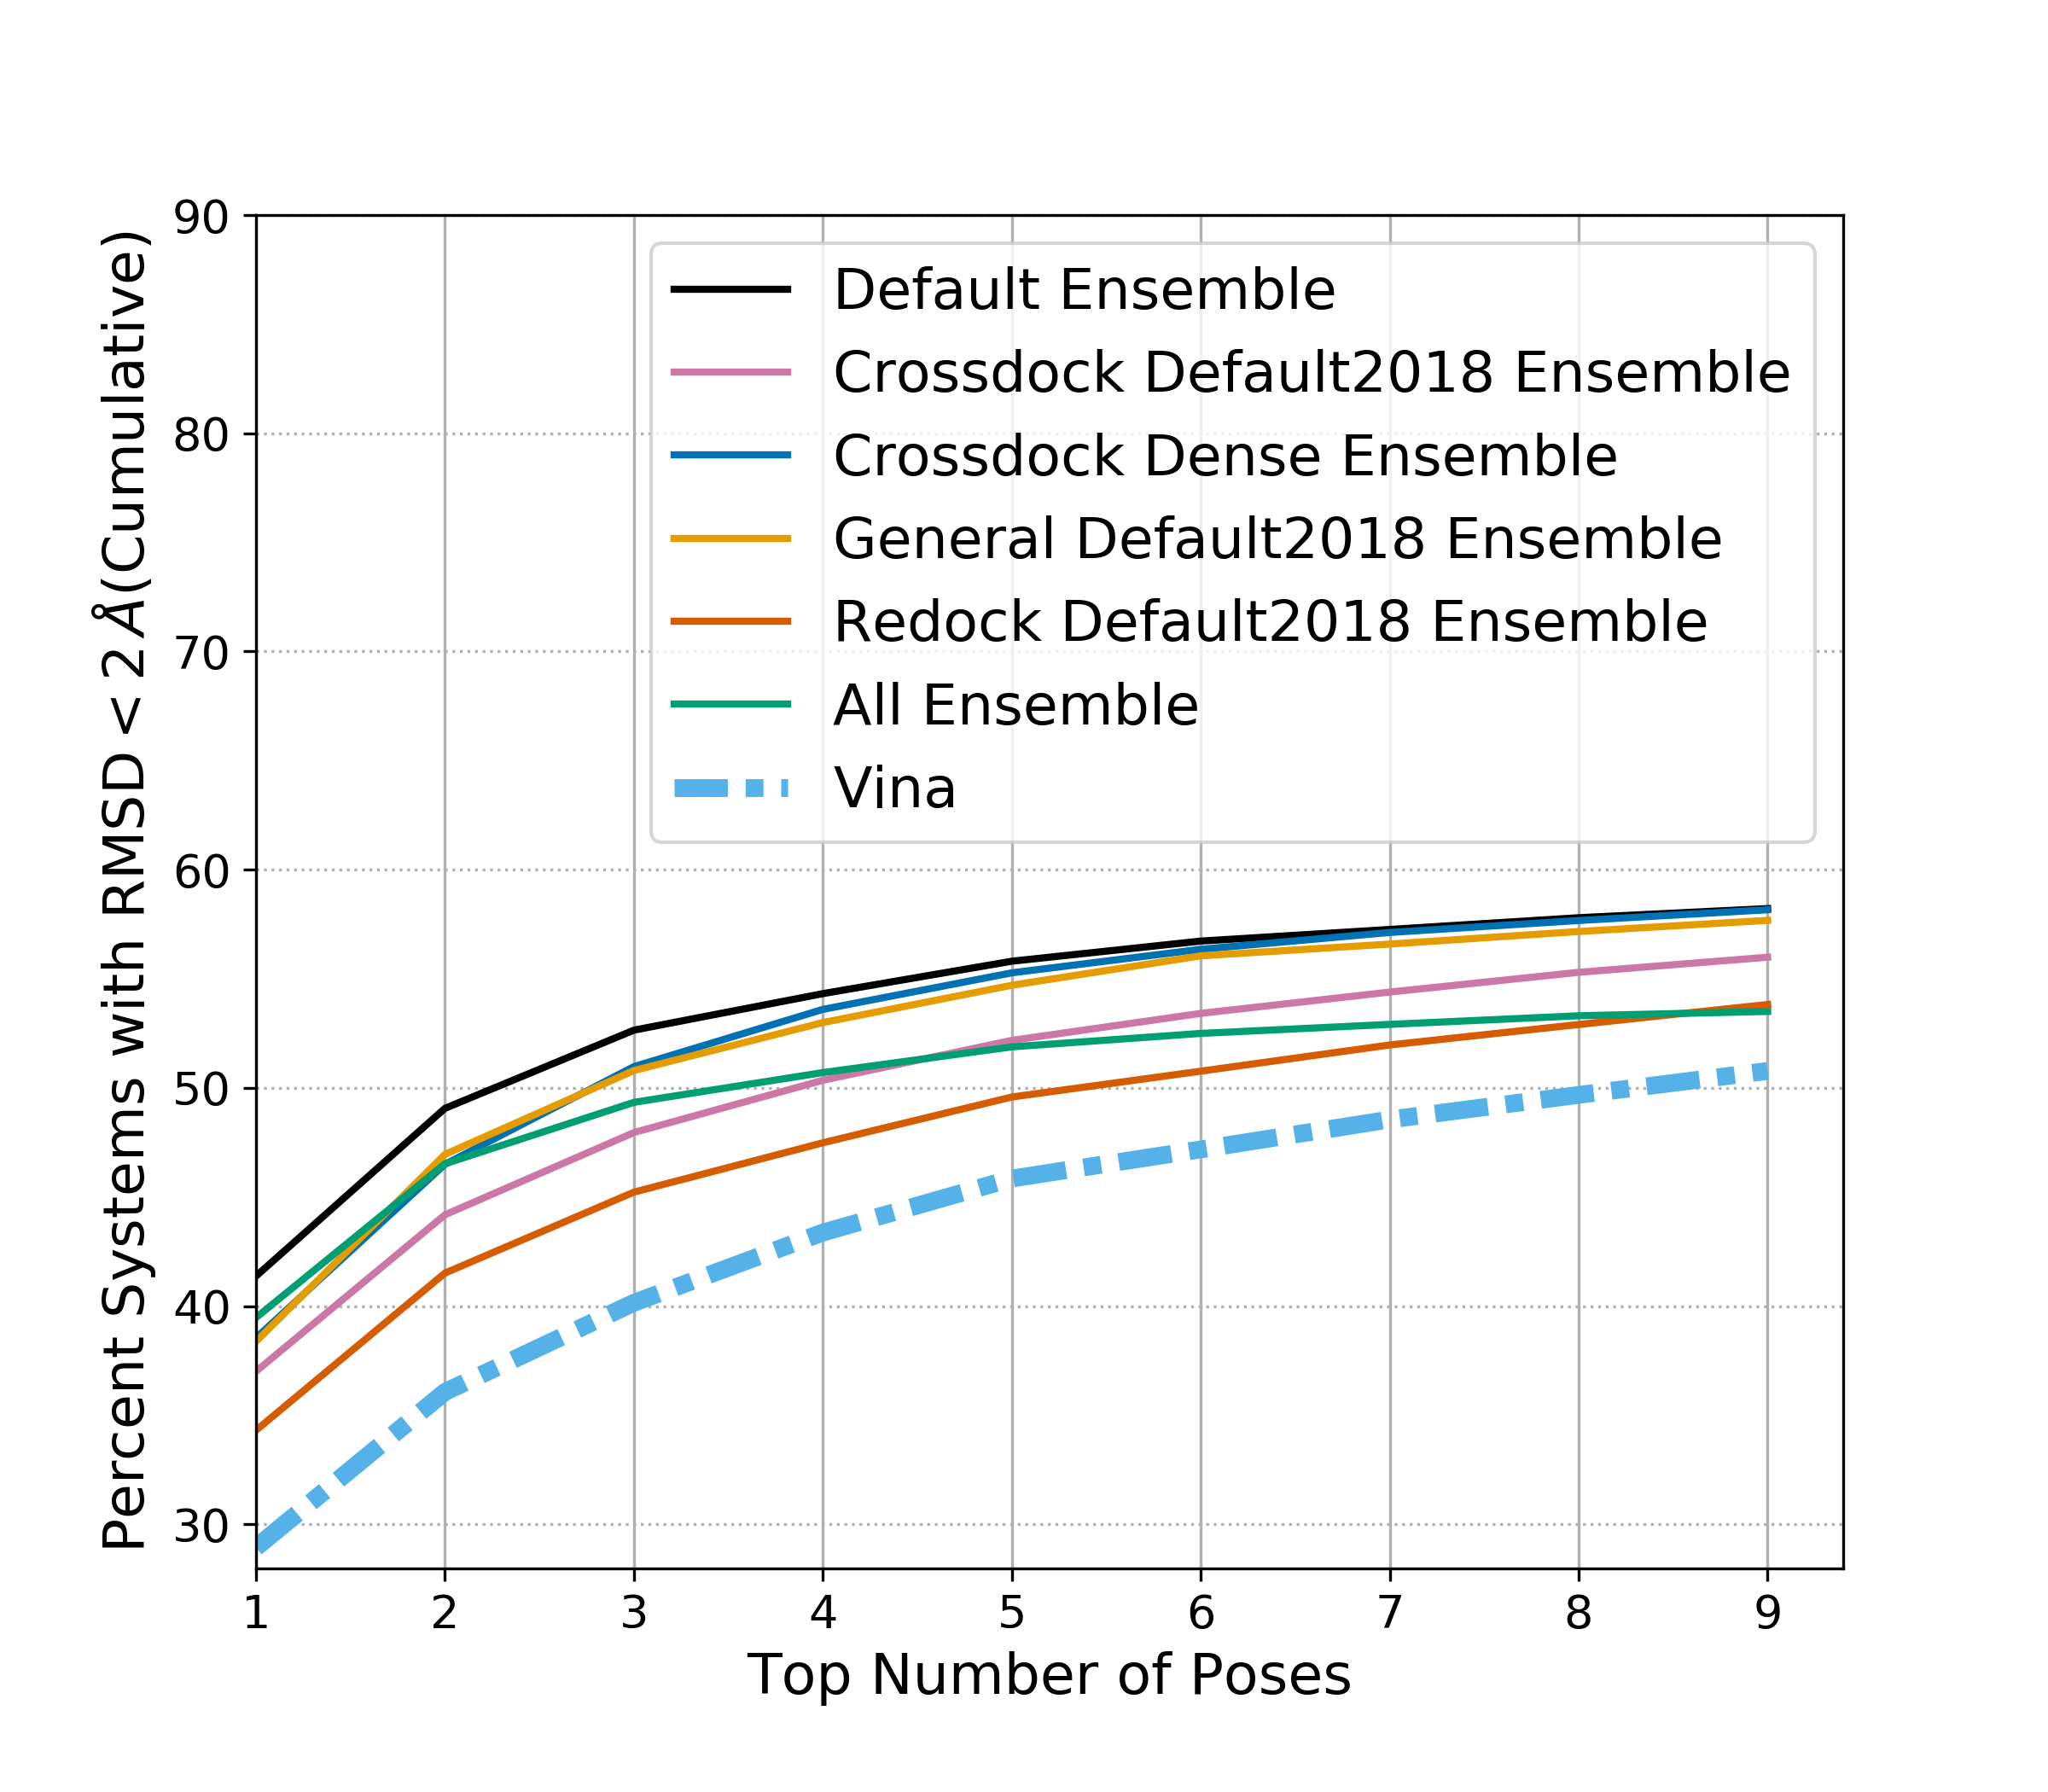
\includegraphics[width=\textwidth]{figures/crossdocking/rescore_ensembles_line.png}
		\caption{Crossdocking}
		\label{fig:resc ens cd}
        \end{subfigure}    
	\caption{Percentage of systems with RMSD to known binding pose less than $2\,\AA$ for each pose with results being cumulative}
	\label{fig:resc ens}
\end{figure}    

\textit{Insert comparison of timings for various ensembles, pareto optimal curve}

\subsection{Optimal Running Method}
When selecting the optimal running method. We evaluate the performance of the Default Ensemble with the "rescore","refinement", and "all" options. However, the usage of the "all" option was unable to complete on the PDBbind Core set in a reasonable amount of time, so it was taken out of consideration. We are then left with comparing the "refinement" and "rescoring" options of the CNN scoring. We can see from \ref{fig:rescore refine comparison} that the Default Ensemble performs nearly equally with either option.

\begin{figure}    
        \begin{subfigure}[b]{0.48\textwidth}    
		\centering
		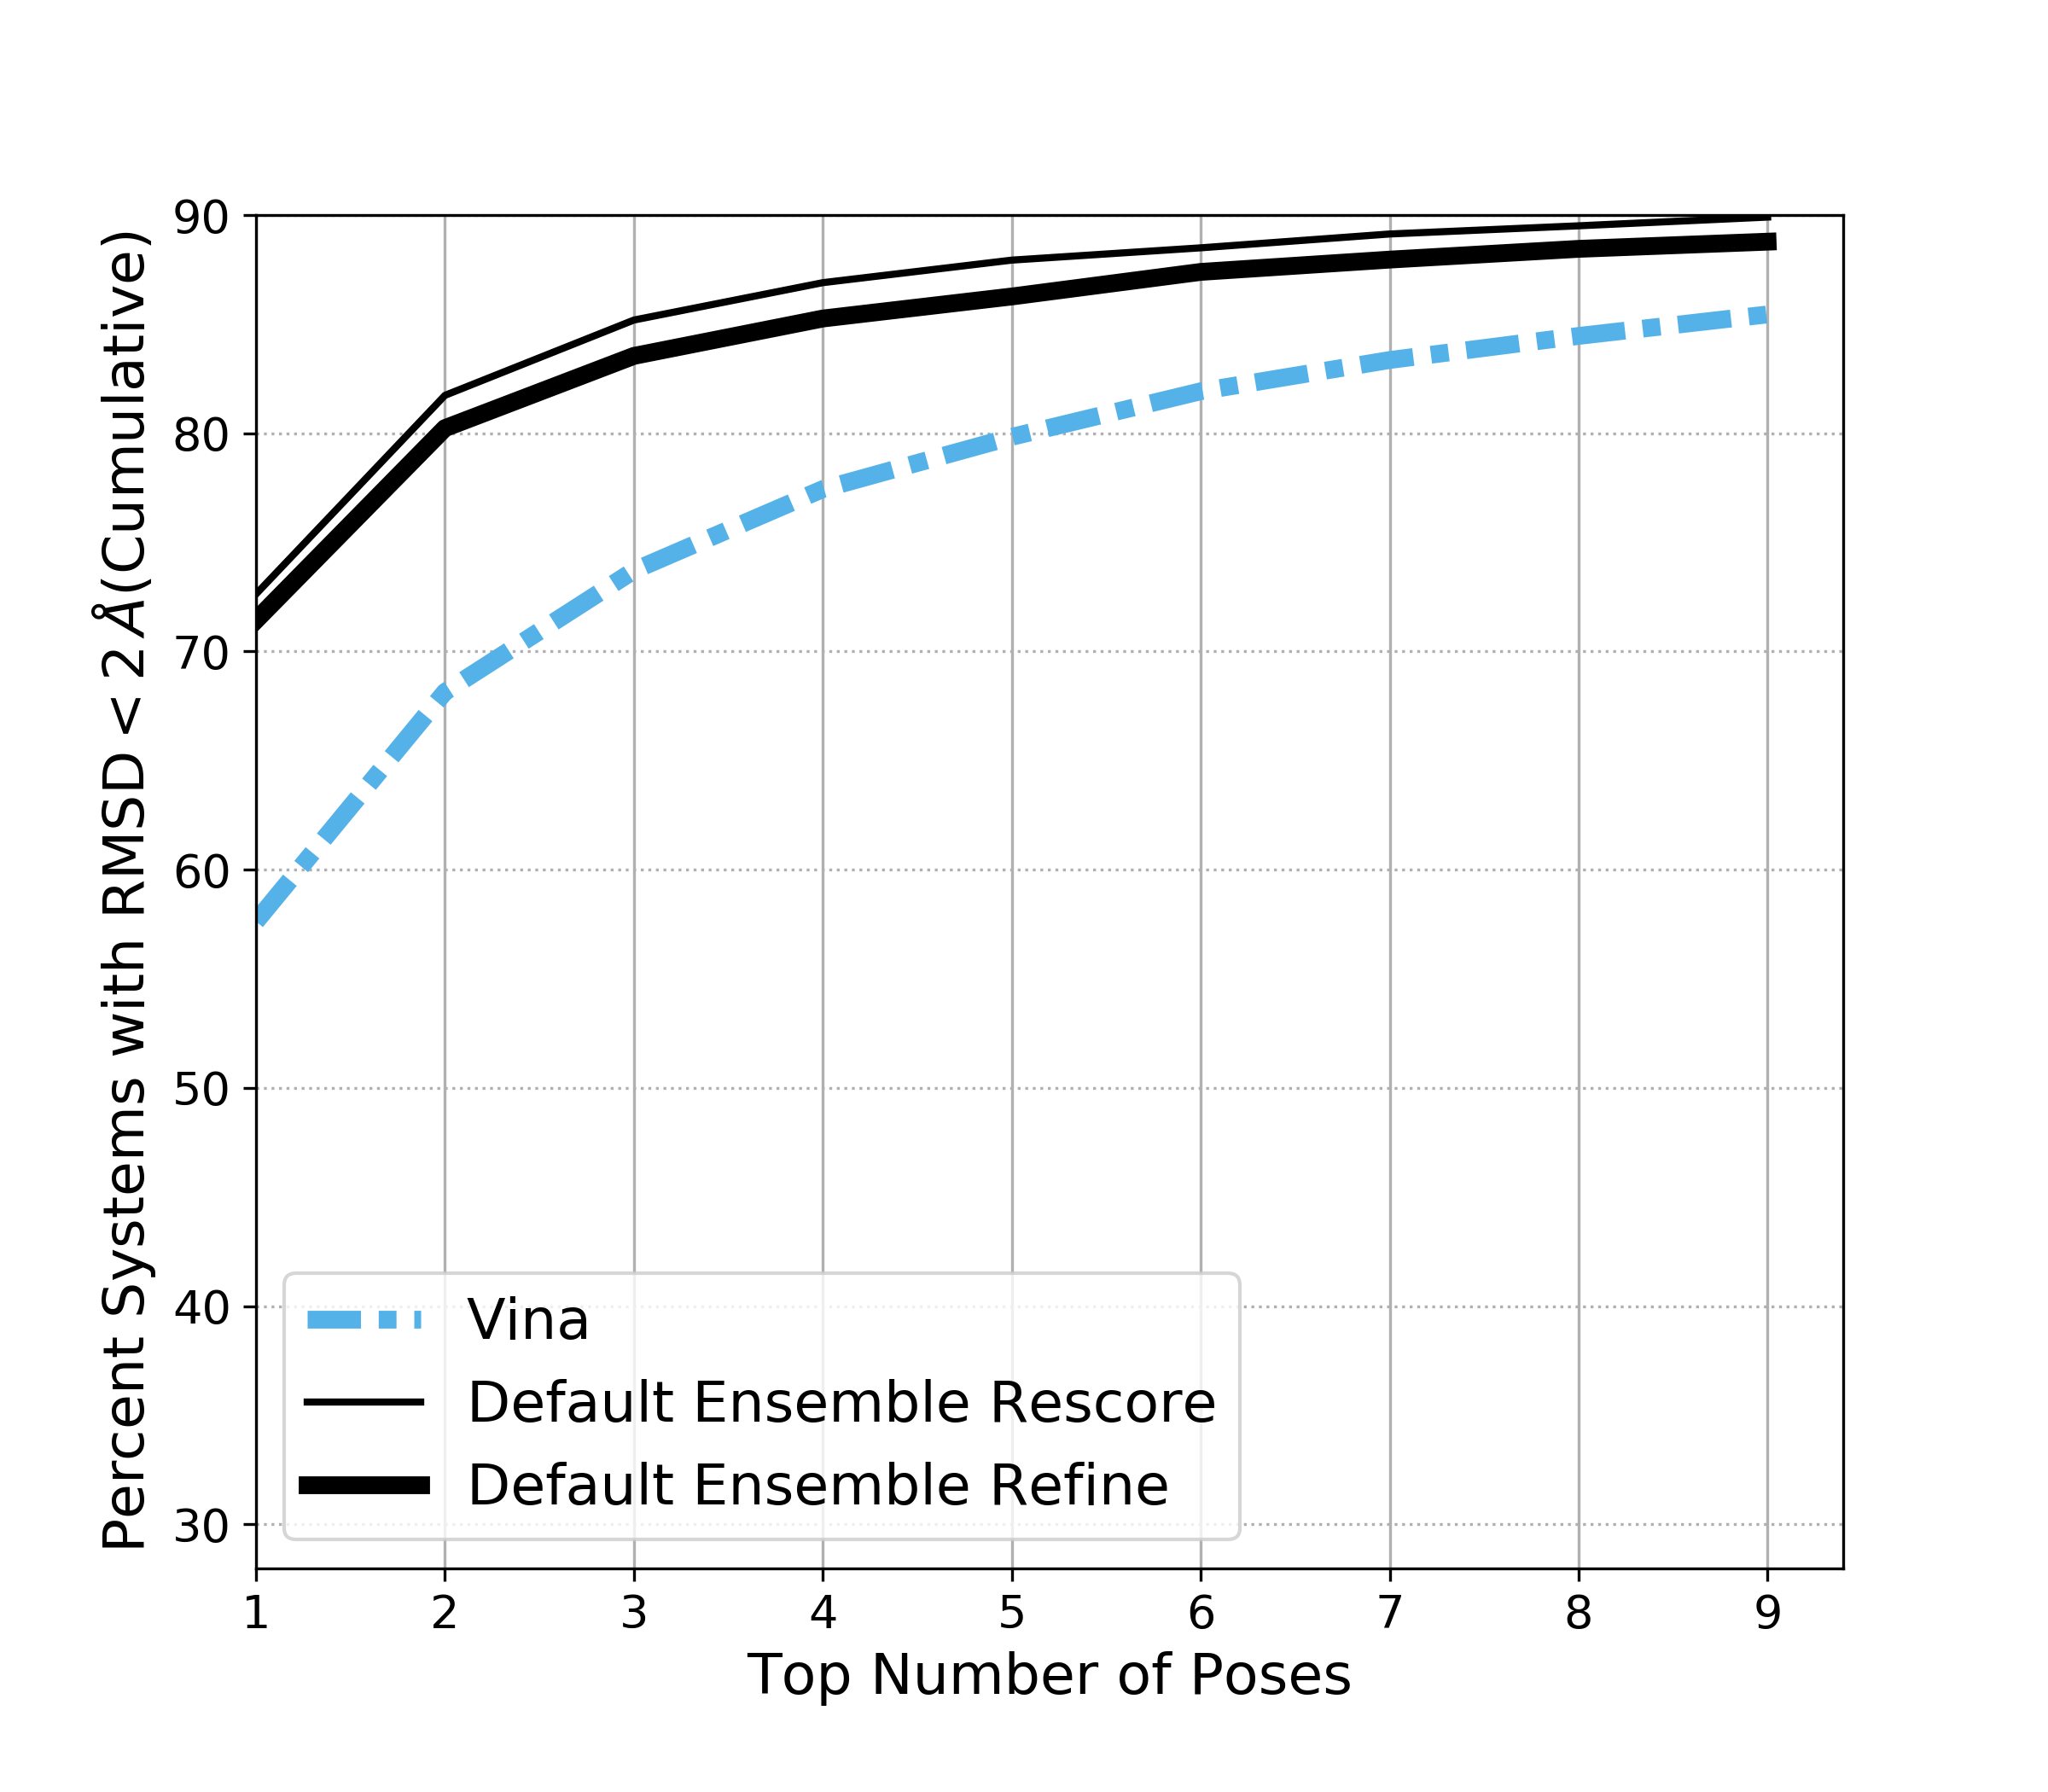
\includegraphics[width=\textwidth]{figures/redocking/rescore_vs_refine_line.png} 
		\caption{Redocking}
		\label{fig:ref vs resc rd}
        \end{subfigure}    
        \begin{subfigure}[b]{0.48\textwidth}    
		\centering
		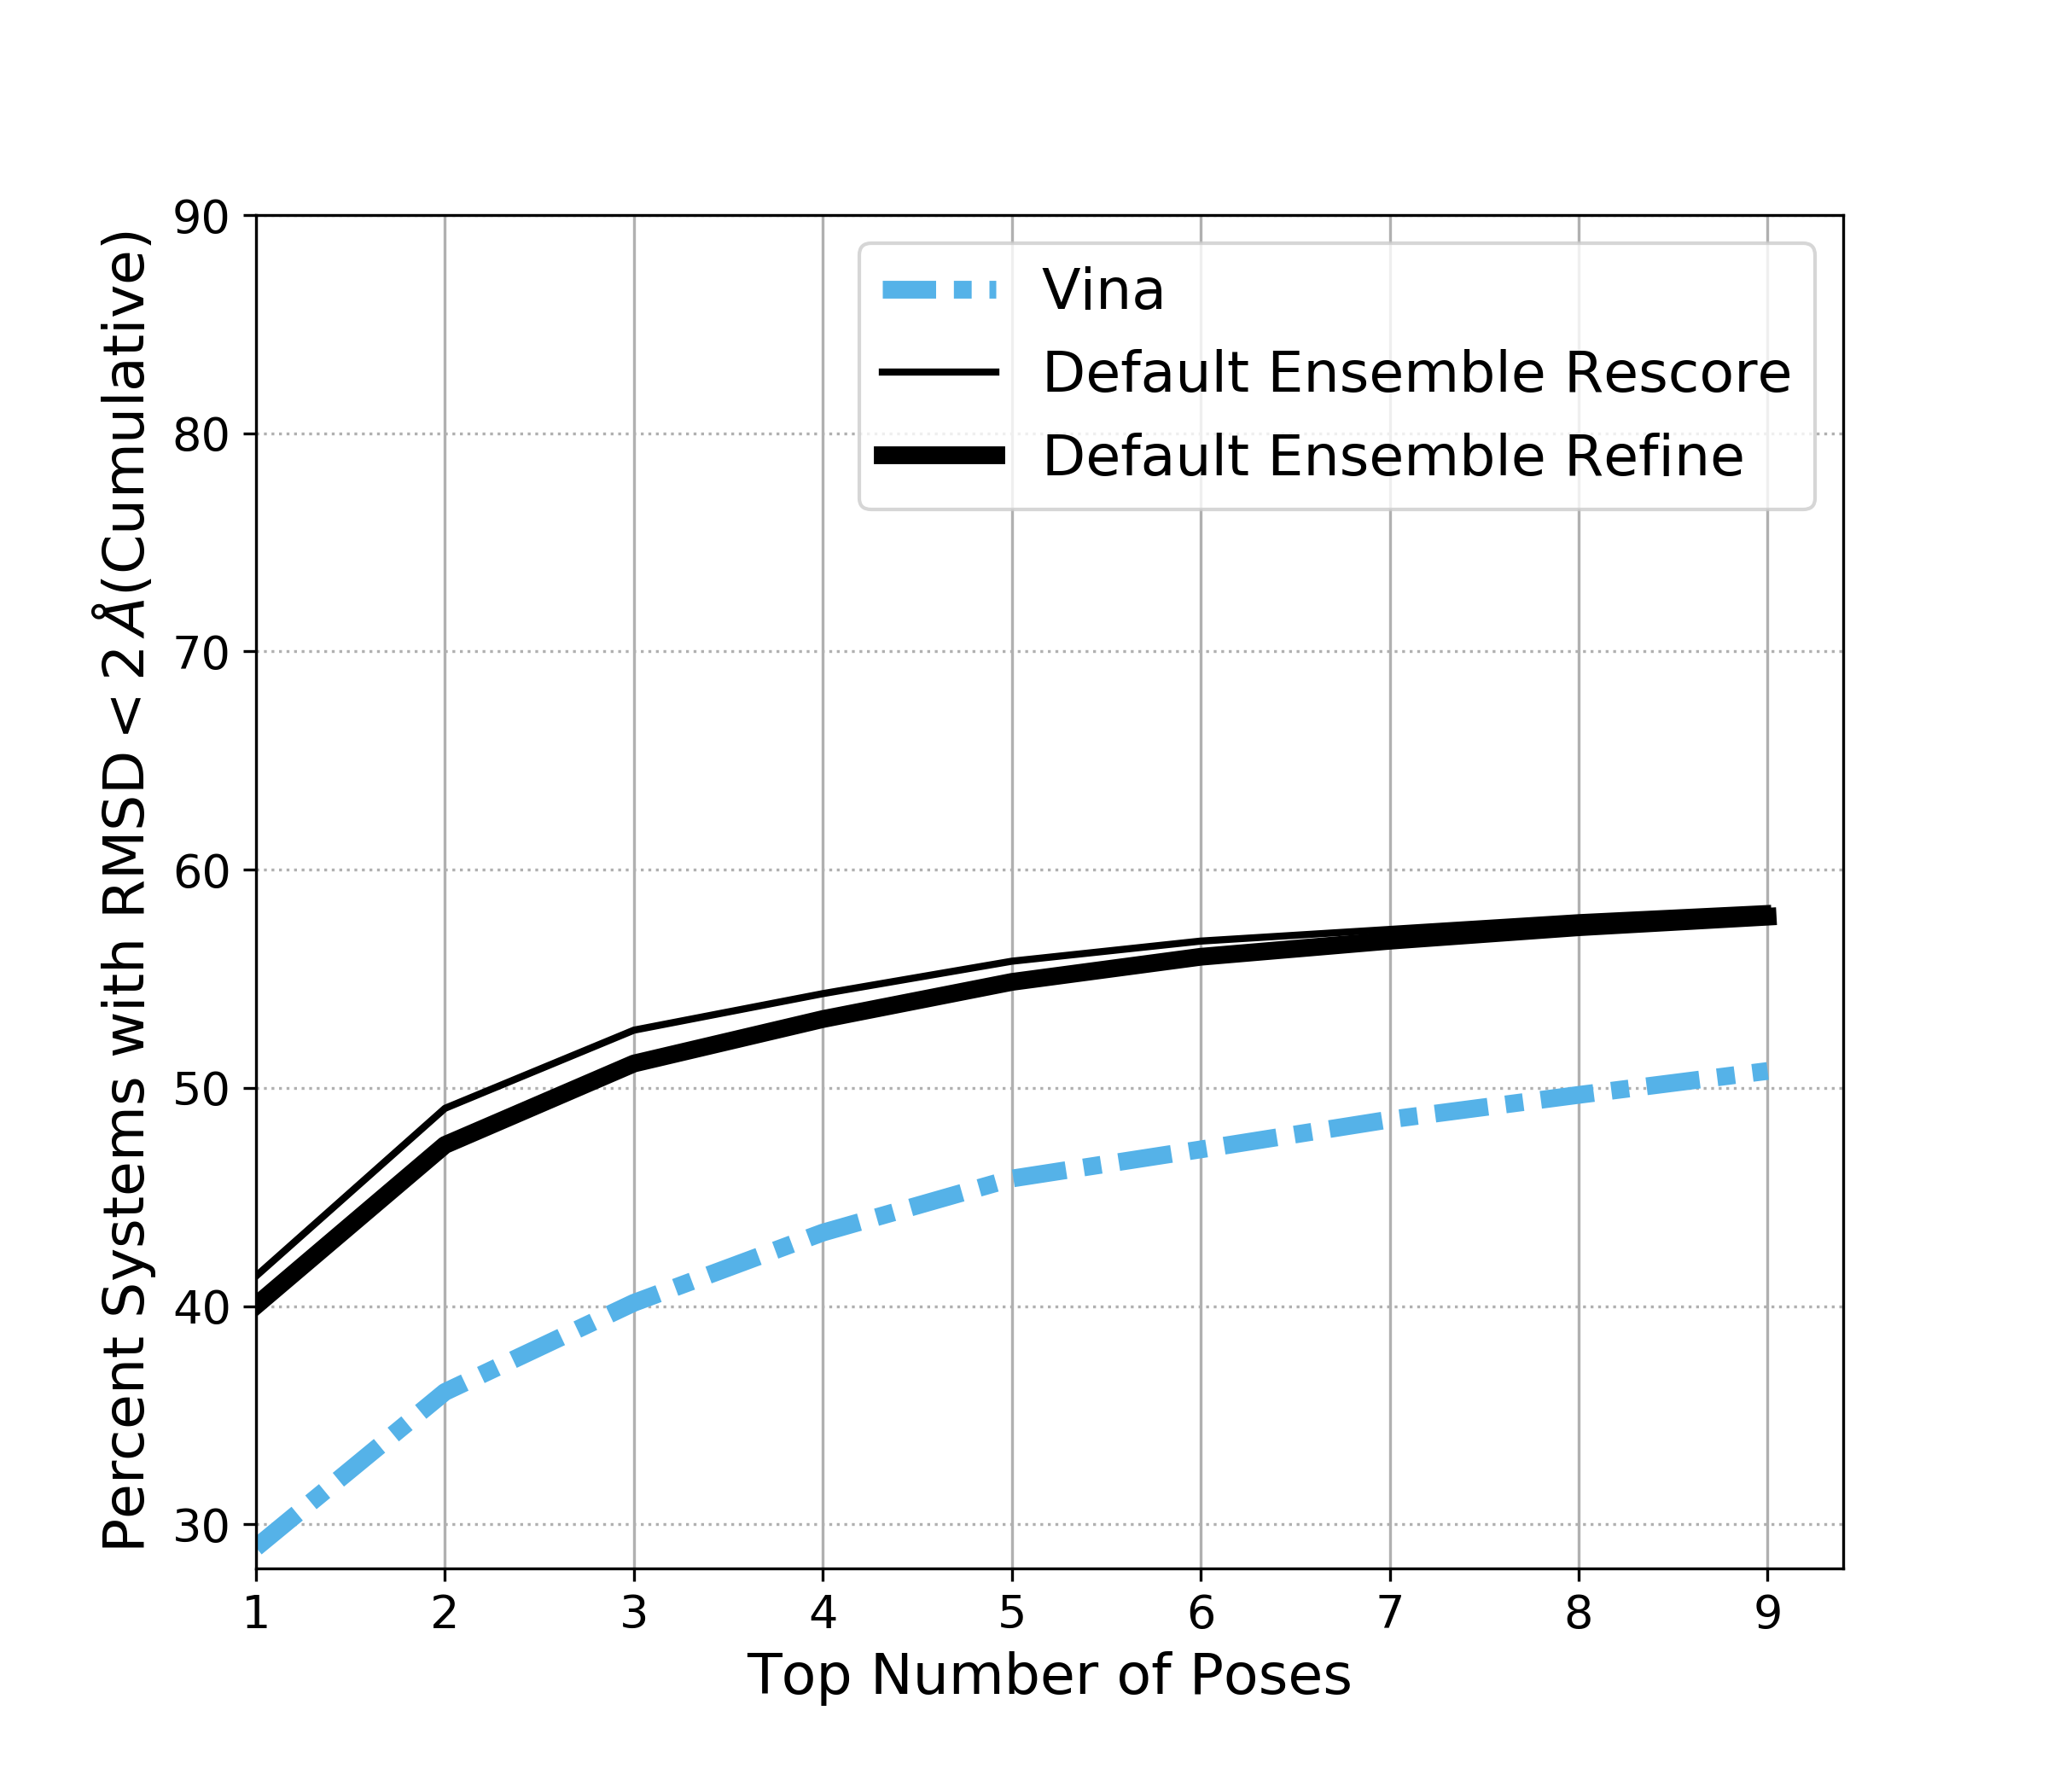
\includegraphics[width=\textwidth]{figures/crossdocking/rescore_vs_refine_line.png} 
		\caption{Crossdocking}
		\label{fig:ref vs resc cd}
        \end{subfigure}    
	\caption{}
	\label{fig:rescore refine comparison}
\end{figure}    

However, from looking at the average time to perform molecular docking for one system. We can see that "refinement" takes significantly longer. Therefore, we select the "rescore" as the default option for the CNN scoring.

\subsection{Settings Exploration}
\begin{figure}    
        \begin{subfigure}[b]{0.48\textwidth}    
		\centering
		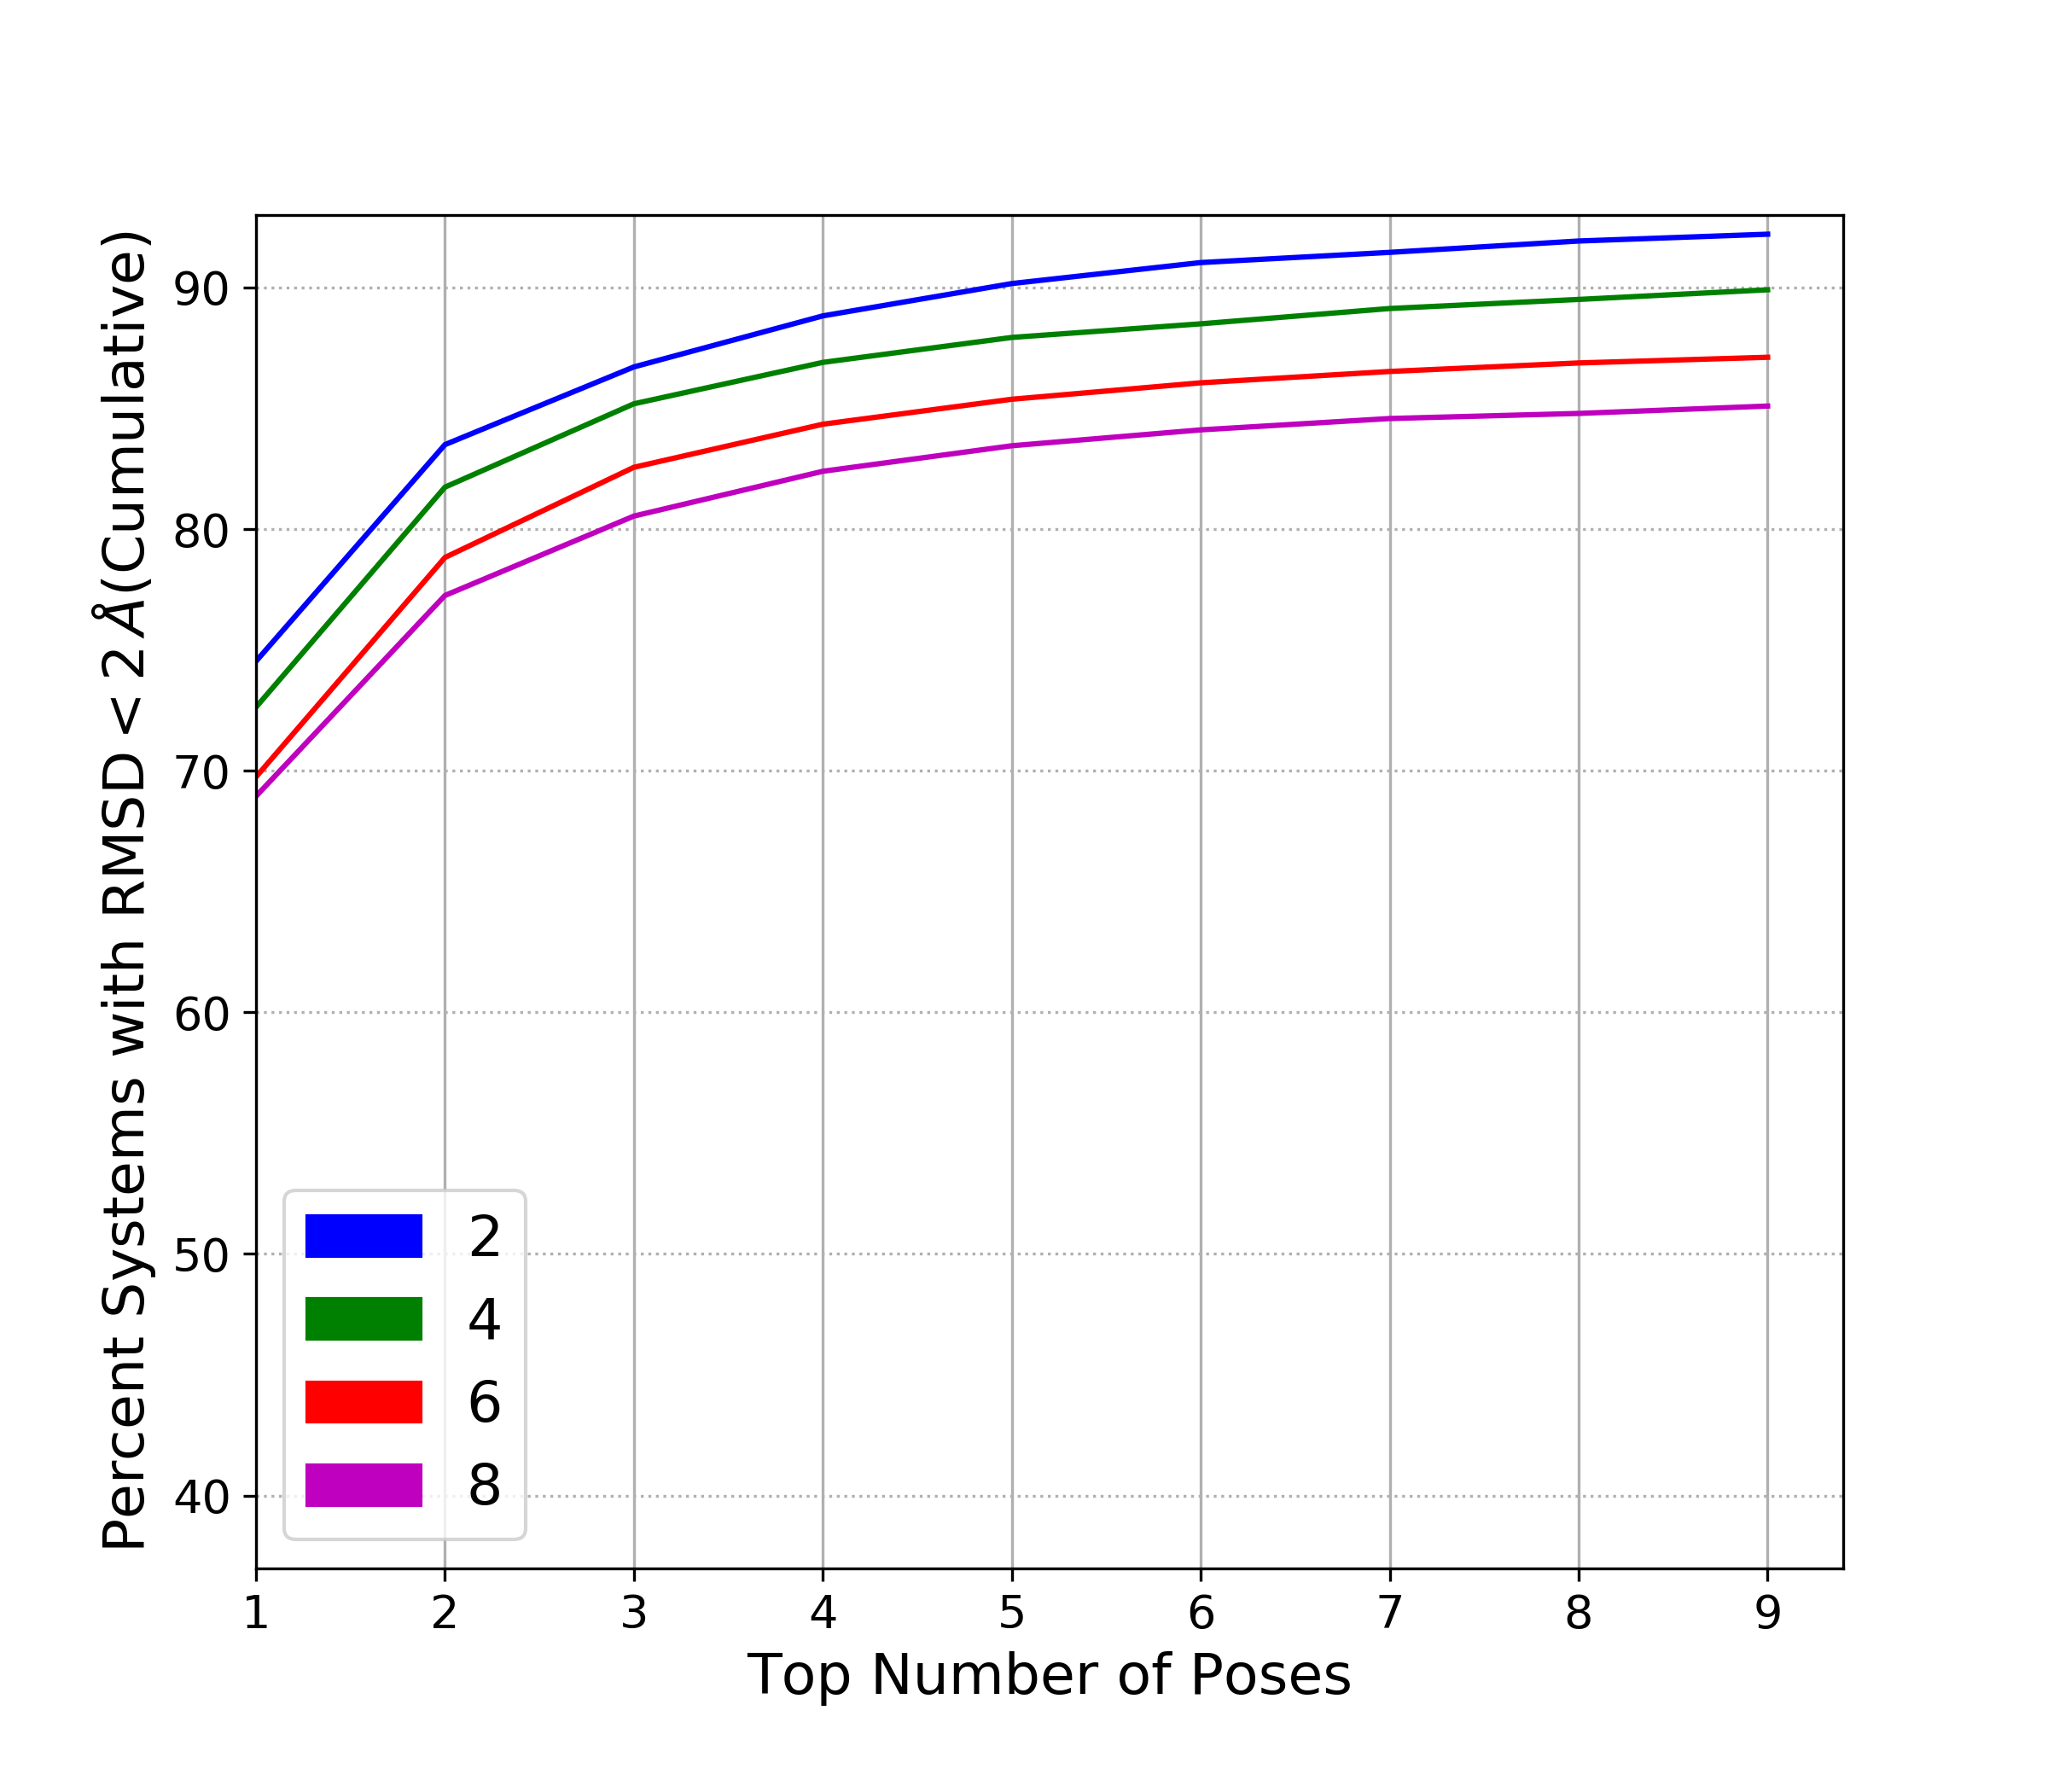
\includegraphics[width=\textwidth]{figures/redocking/sweep_autobox_add_line.png}
		\caption{Redocking}
		\label{fig:autobox add rd}
        \end{subfigure}    
        \begin{subfigure}[b]{0.48\textwidth}    
		\centering
		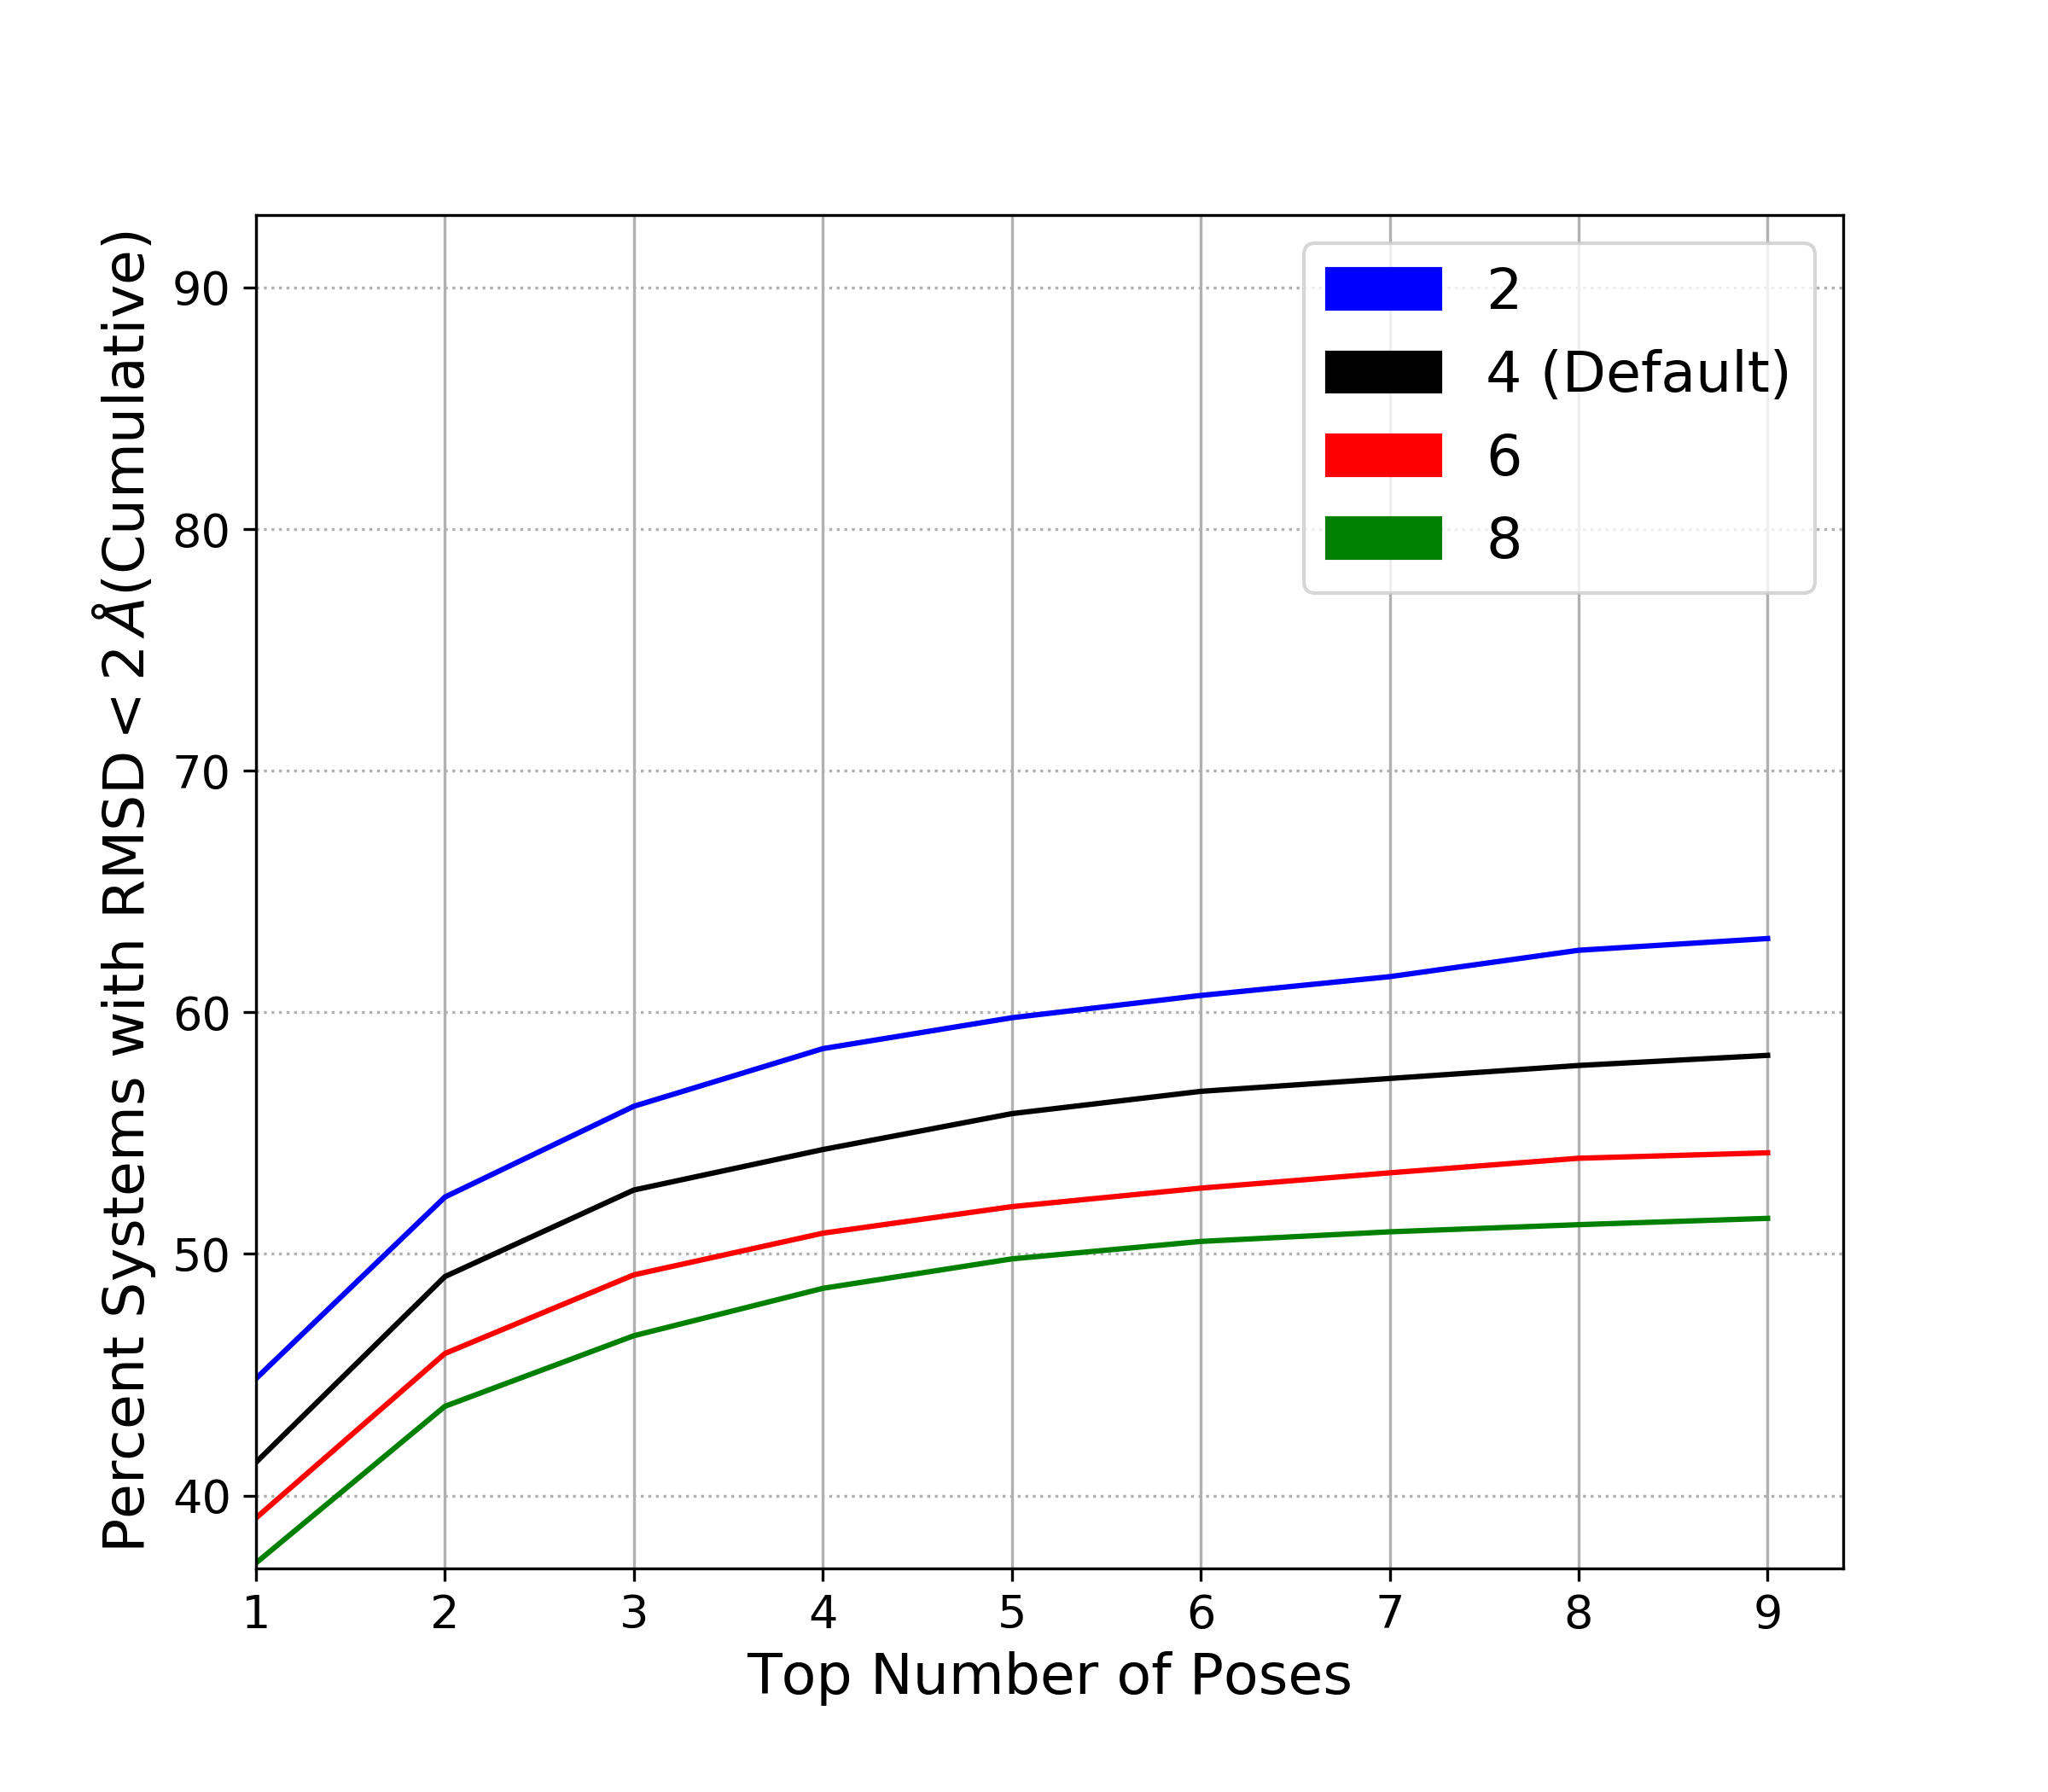
\includegraphics[width=\textwidth]{figures/crossdocking/sweep_autobox_add_line.png}
		\caption{Crossdocking}
		\label{fig:autobox add cd}
        \end{subfigure}    
	\caption{}
	\label{fig:autobox add}
\end{figure}    
First we evaluate all of the settings for defined pockets. Autobox add increases the search space for the docking program to be larger than the rectangular prism defined by the autobox ligand input to Gnina by the given value on each side. In redocking, the expansion of the search space decreases performance as the docking box provided by autobox ligand is exactly where the ligand should be. Crossdocking is a different story as the new ligand might fit in a different area of the defined pocket.

\begin{figure}    
        \begin{subfigure}[b]{0.48\textwidth}    
		\centering
		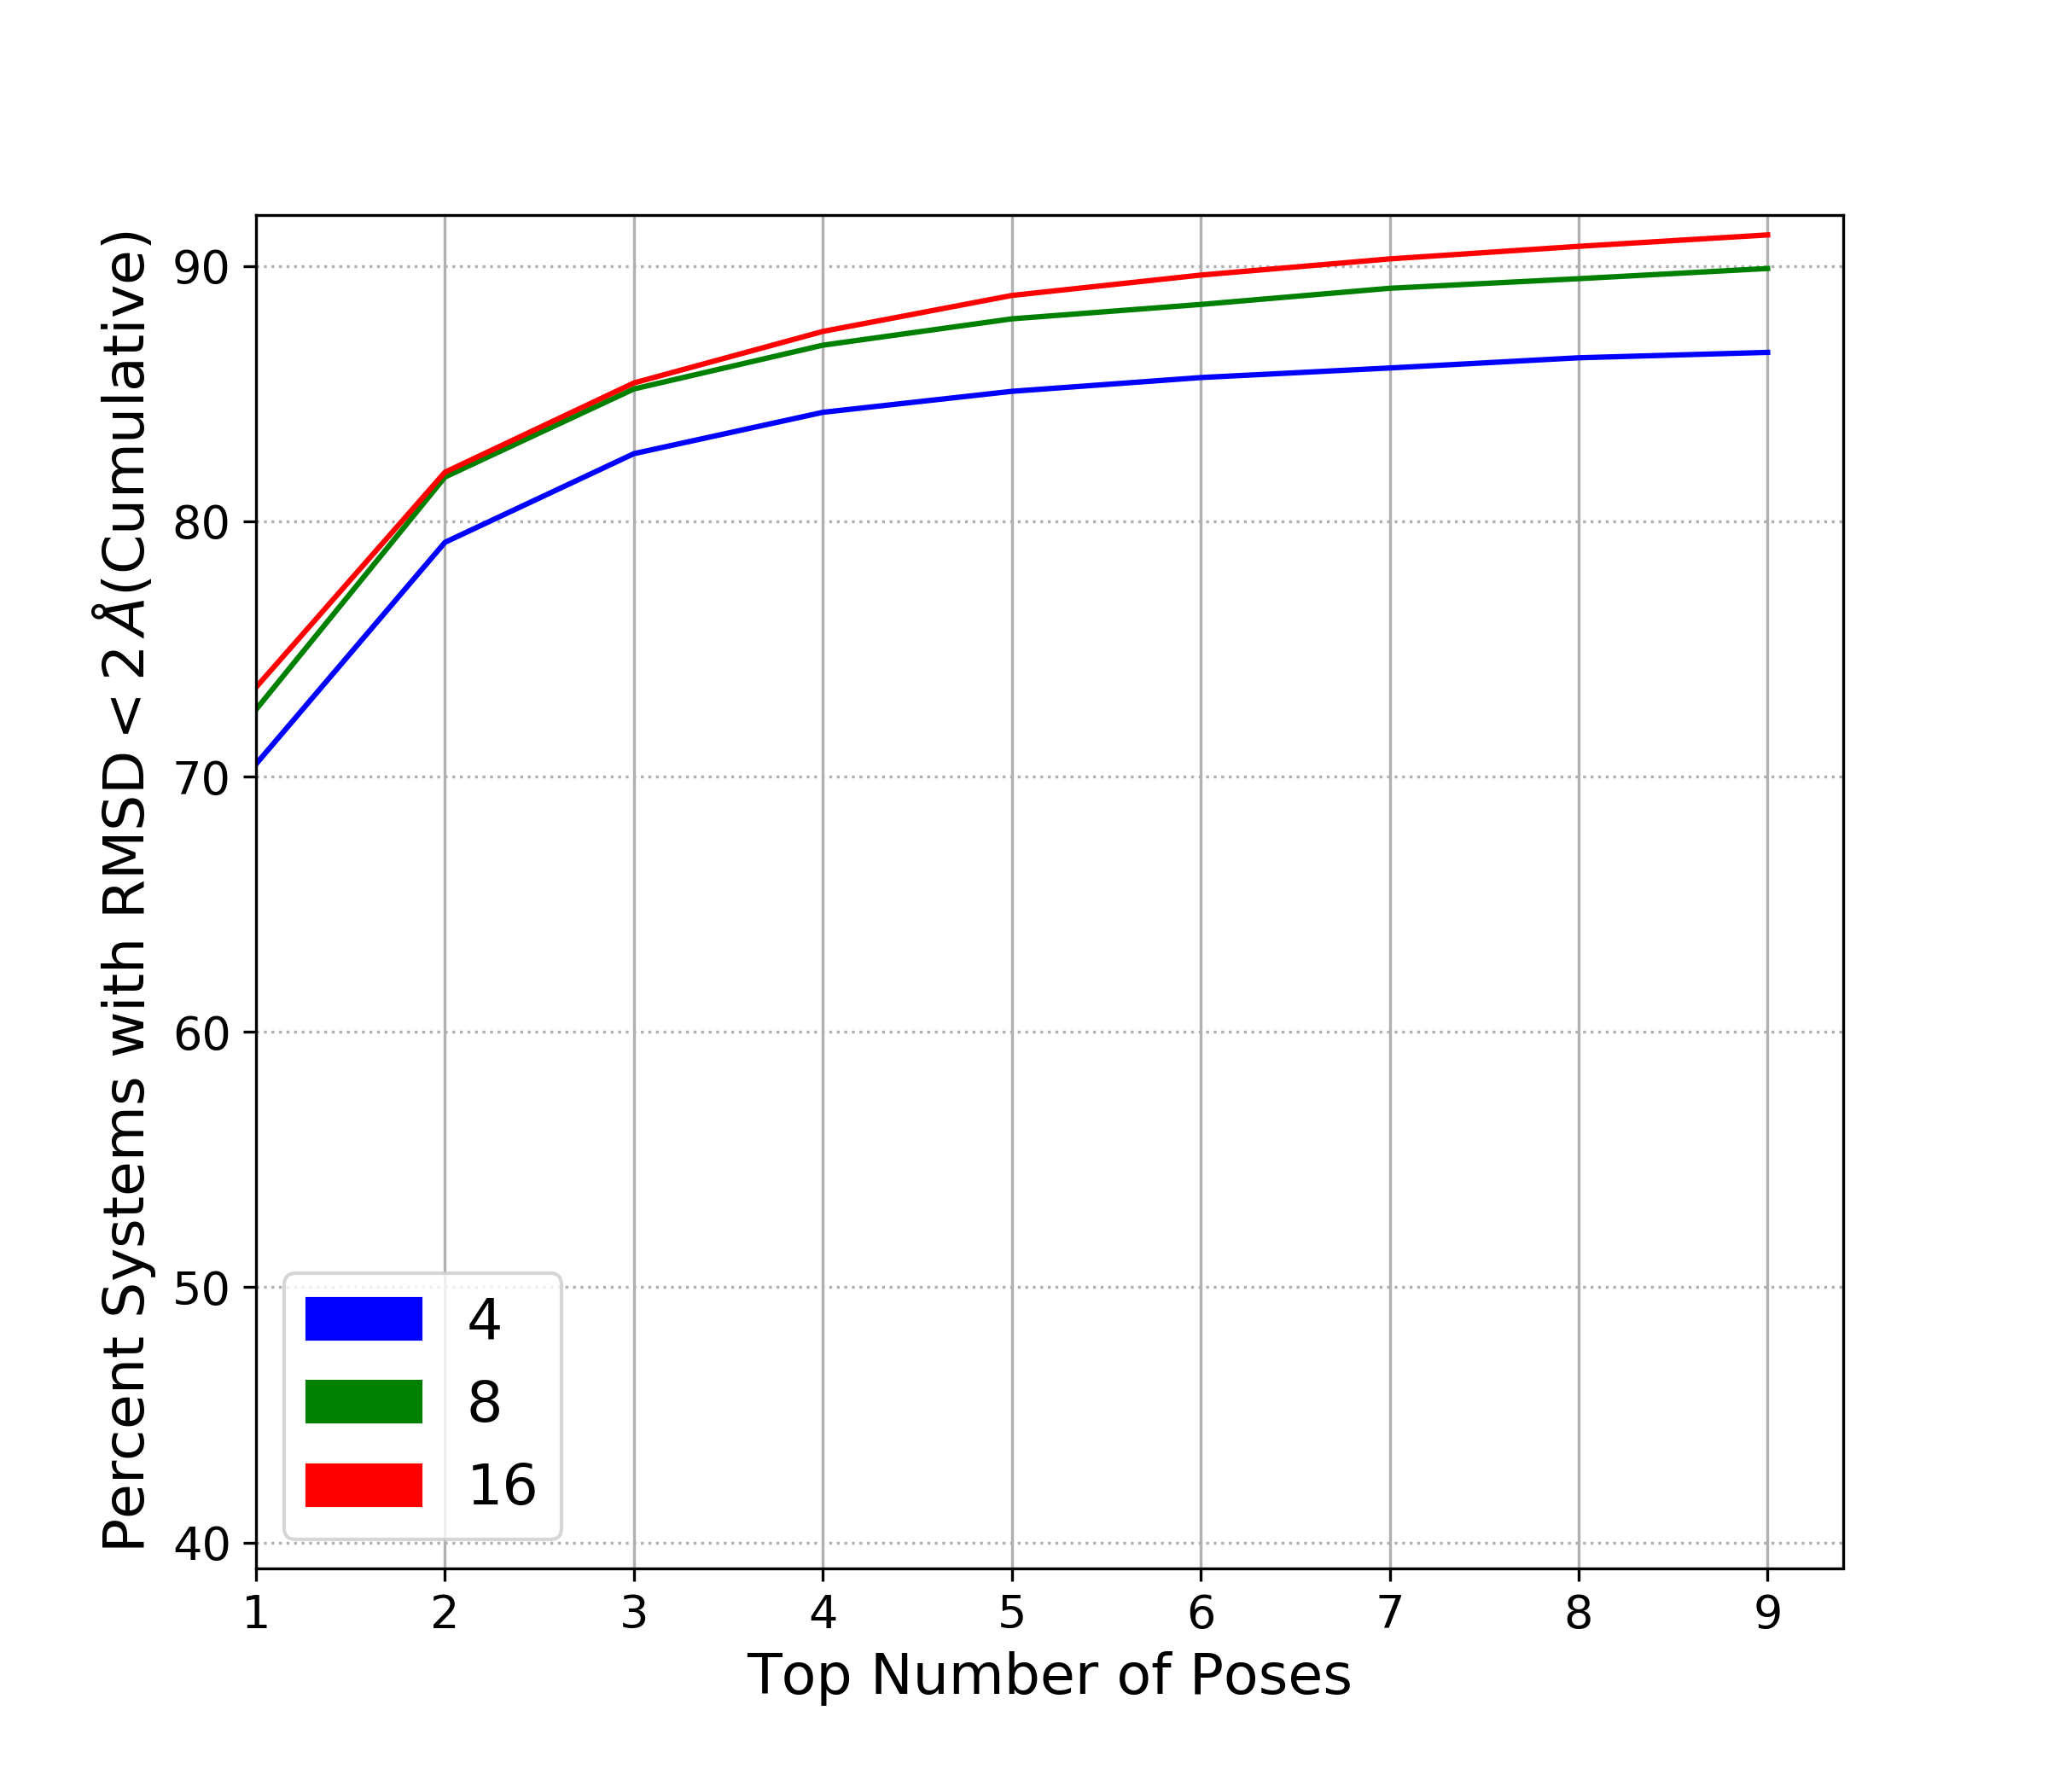
\includegraphics[width=\textwidth]{figures/redocking/sweep_exhaustiveness_line.png}
		\caption{Redocking}
		\label{fig:exhaustiveness rd}
        \end{subfigure}    
        \begin{subfigure}[b]{0.48\textwidth}    
		\centering
		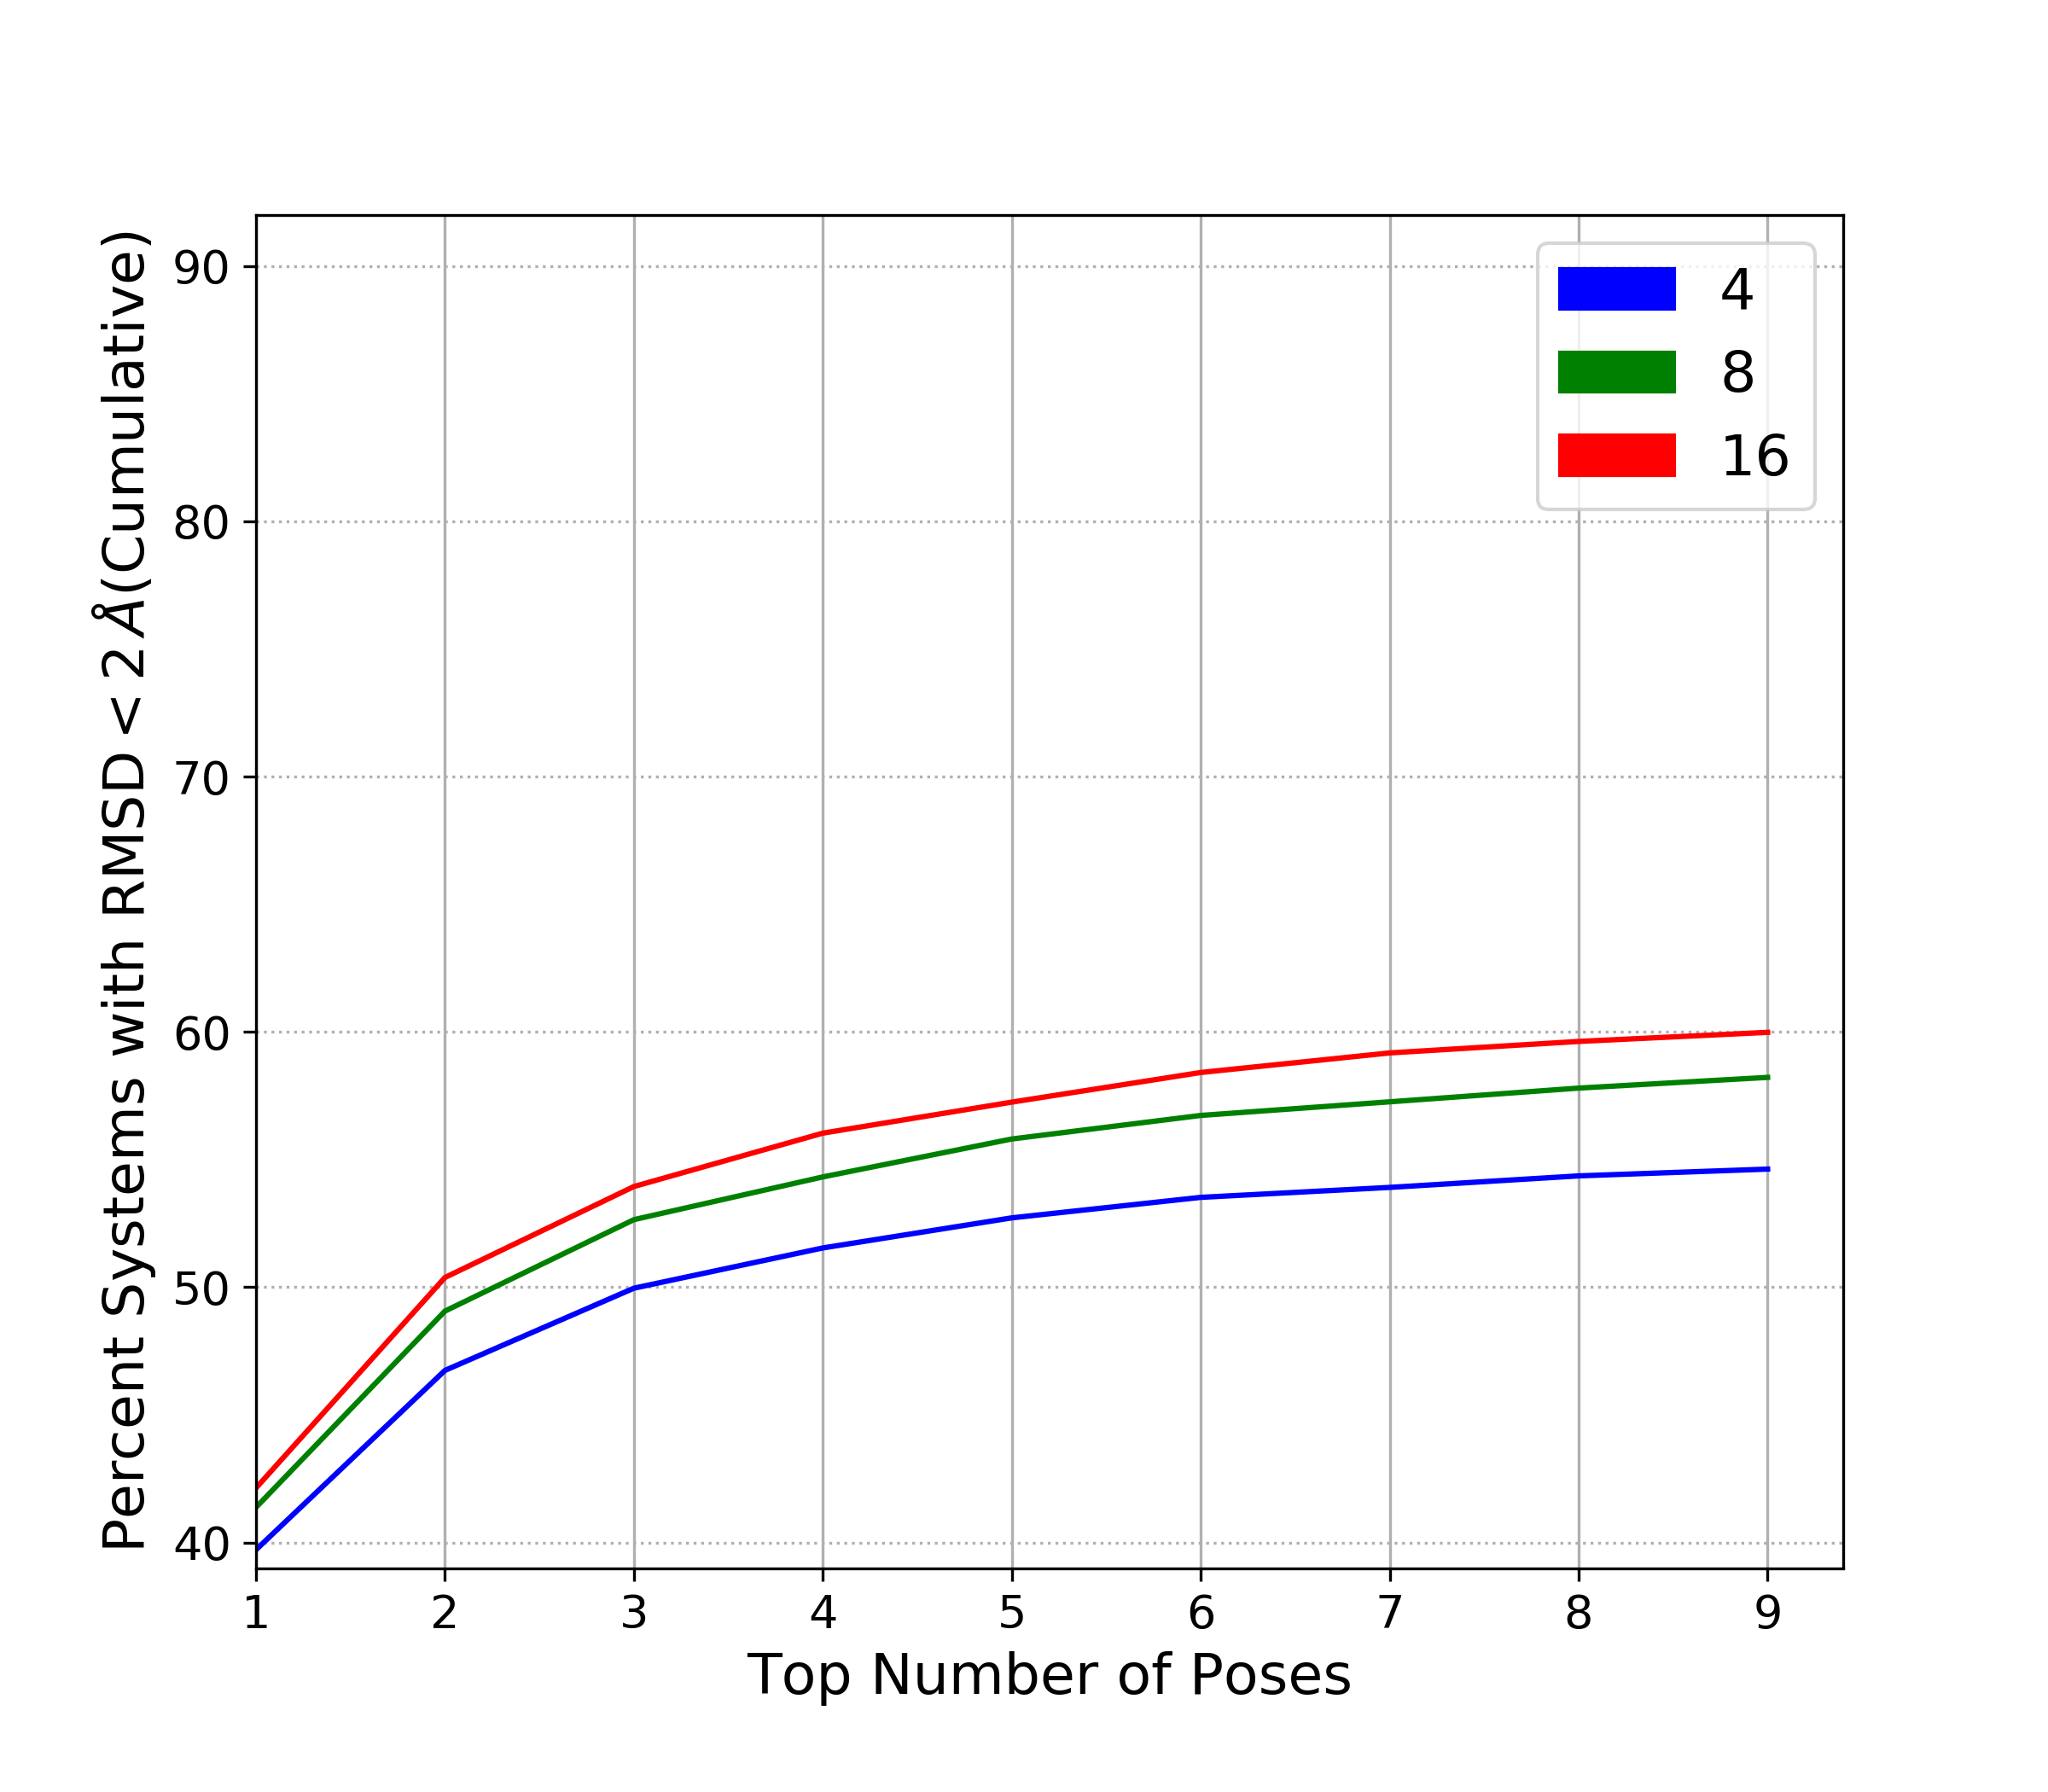
\includegraphics[width=\textwidth]{figures/crossdocking/sweep_exhaustiveness_line.png}
		\caption{Crossdocking}
		\label{fig:exhaustiveness cd}
        \end{subfigure}    
	\caption{}
	\label{fig:exhaustiveness}
\end{figure}    

Changes in the exhaustiveness alter the amount of sampling that occurs. When the exhaustiveness is increased, we see an increase in the performance of the docking. This is as expected, more monte carlo chains randomly mutating the ligand conformation provides the docking procedure with more opportunities to randomly sample the correct answer. However, we this increase in performance seems to reach limited gains after the value of 8. An exhaustiveness of 16 provides some performance boost, but this boost is accompanied by a doubling of the compuational time. The monte carlo chains are evaluated in a parallel manner, but this is limited by the number of cores available to Gnina. So if the exhaustiveness is greater than the cpus provided to Gnina, the number of simultaneously running monte carlo chains is equal to the number of cpus. Therefore, in typical usage of Gnina, an exhaustiveness level of 8 is sufficient for adequate performance levels while minimizing the computational load.

\begin{figure}    
        \begin{subfigure}[b]{0.48\textwidth}    
		\centering
		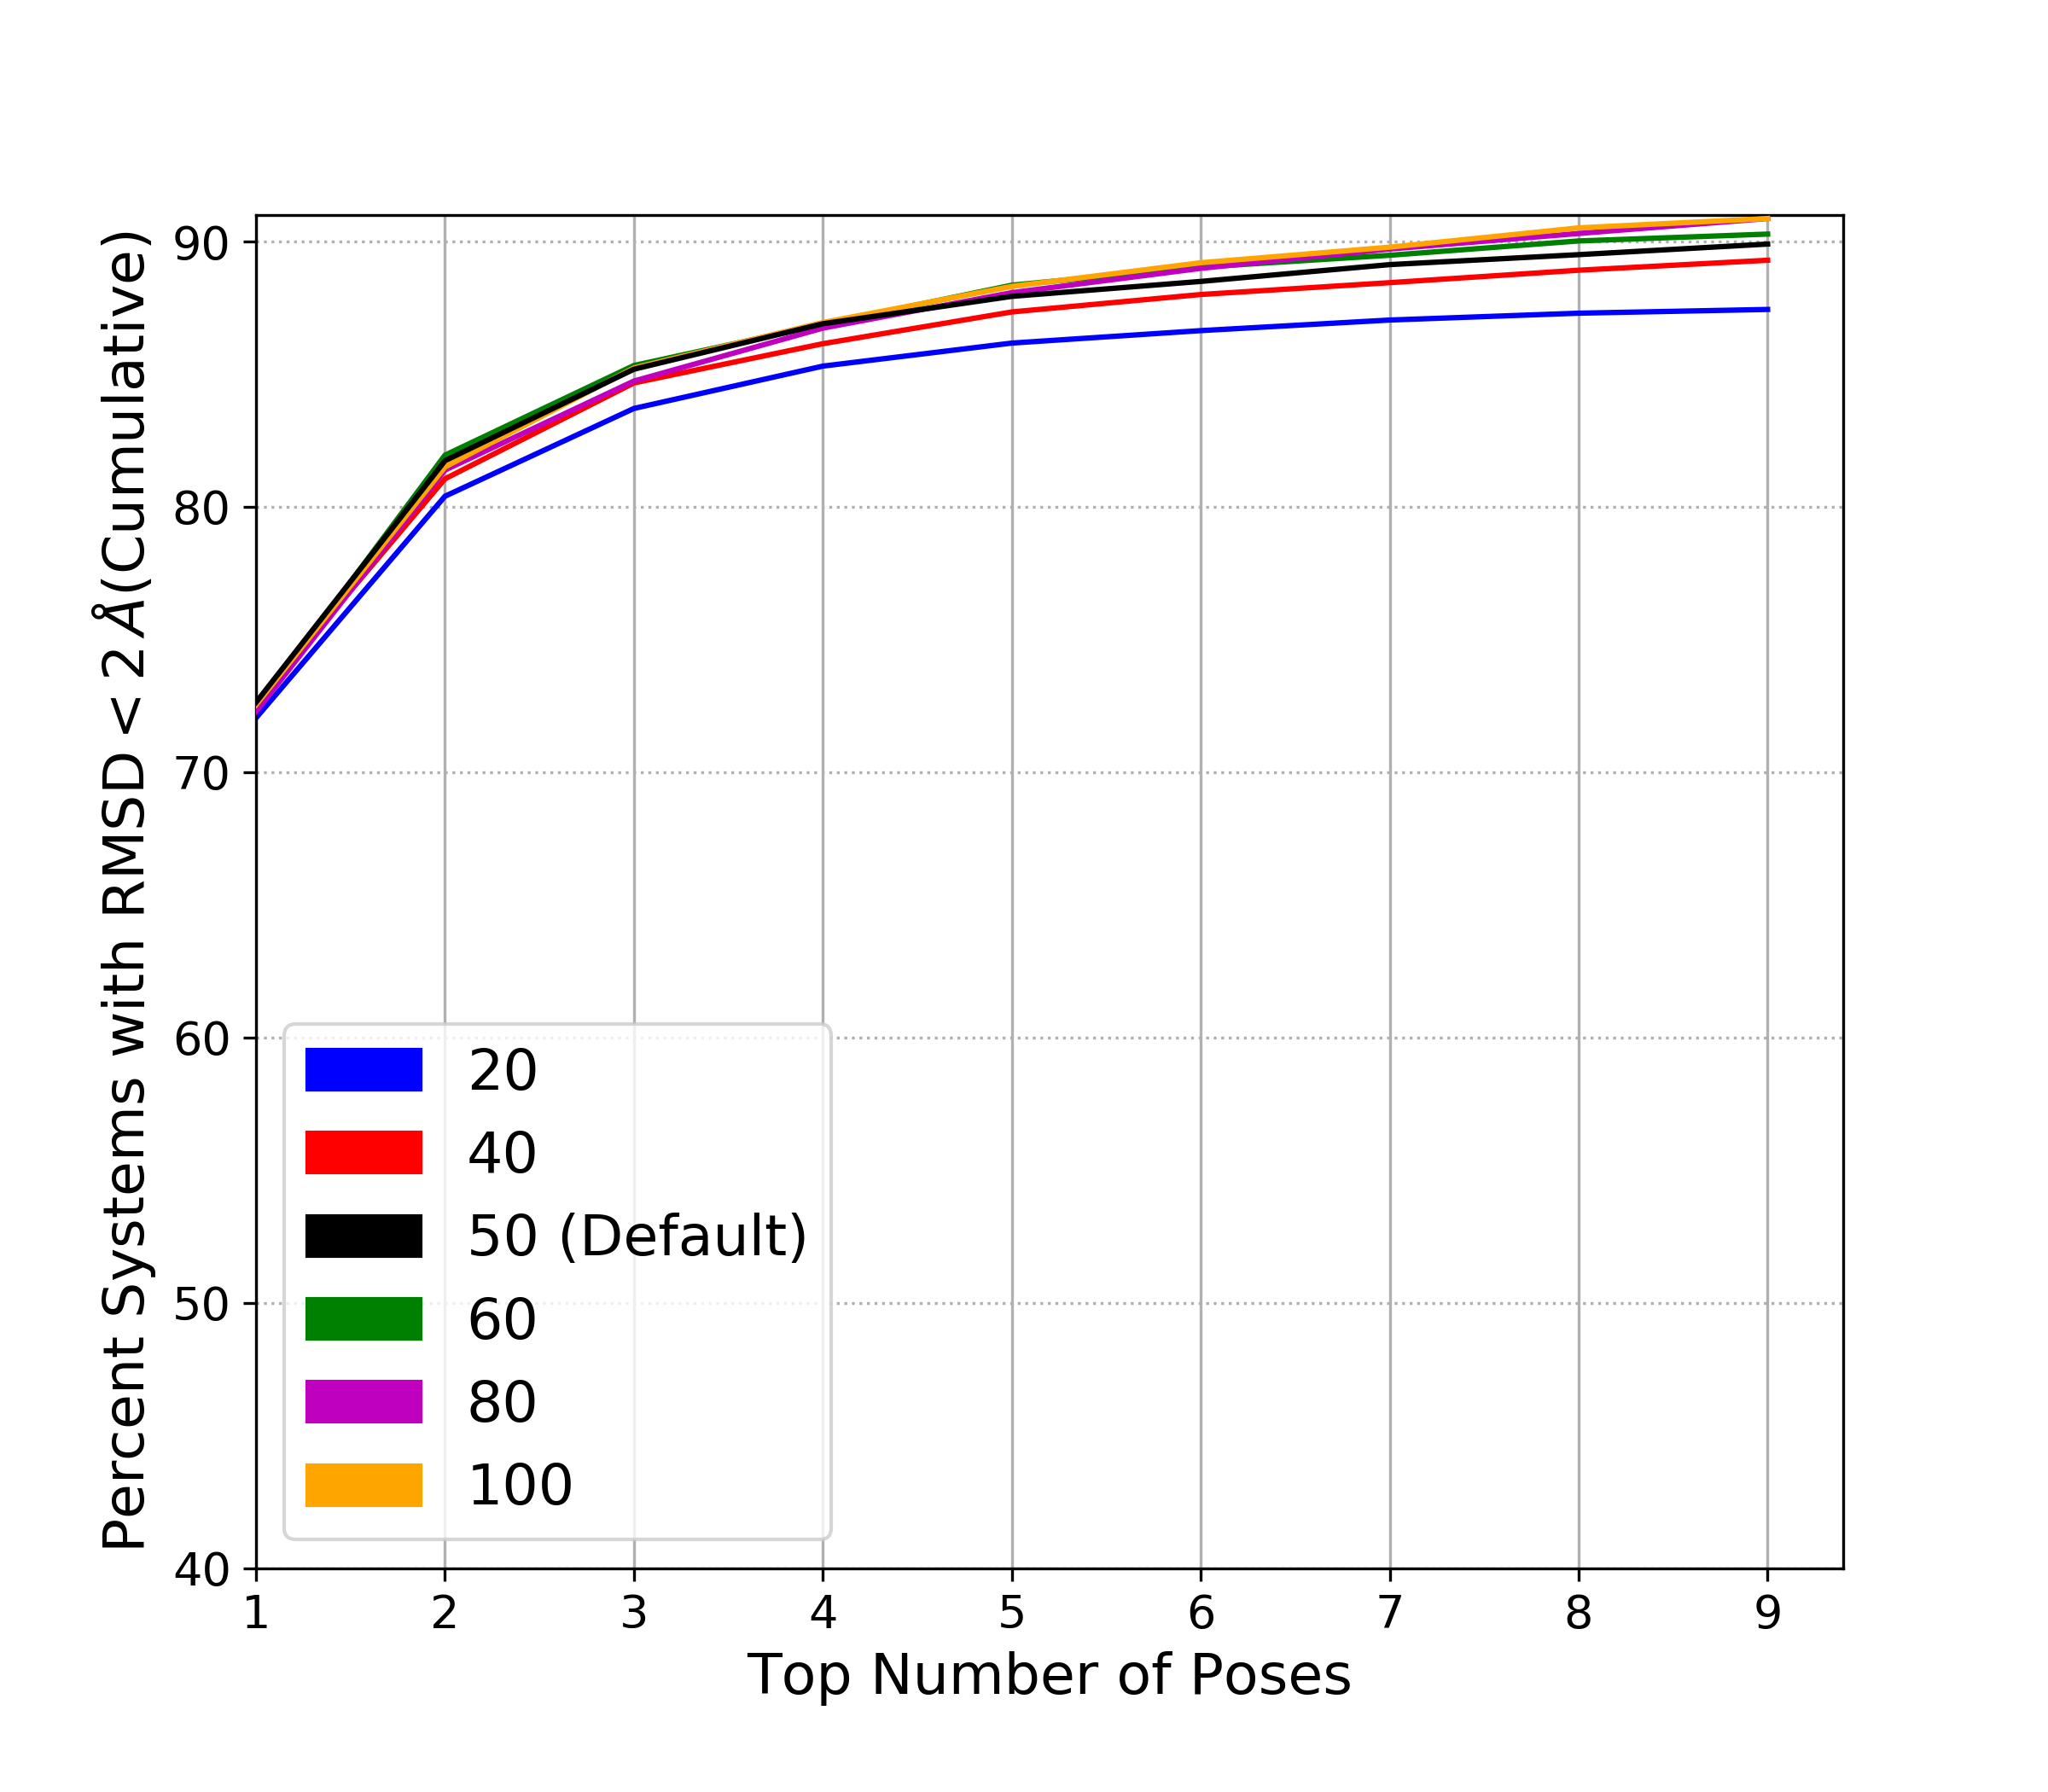
\includegraphics[width=\textwidth]{figures/redocking/sweep_mcsaved_line.png}
		\caption{Redocking}
		\label{fig:mcsaved rd}
        \end{subfigure}    
        \begin{subfigure}[b]{0.48\textwidth}    
		\centering
		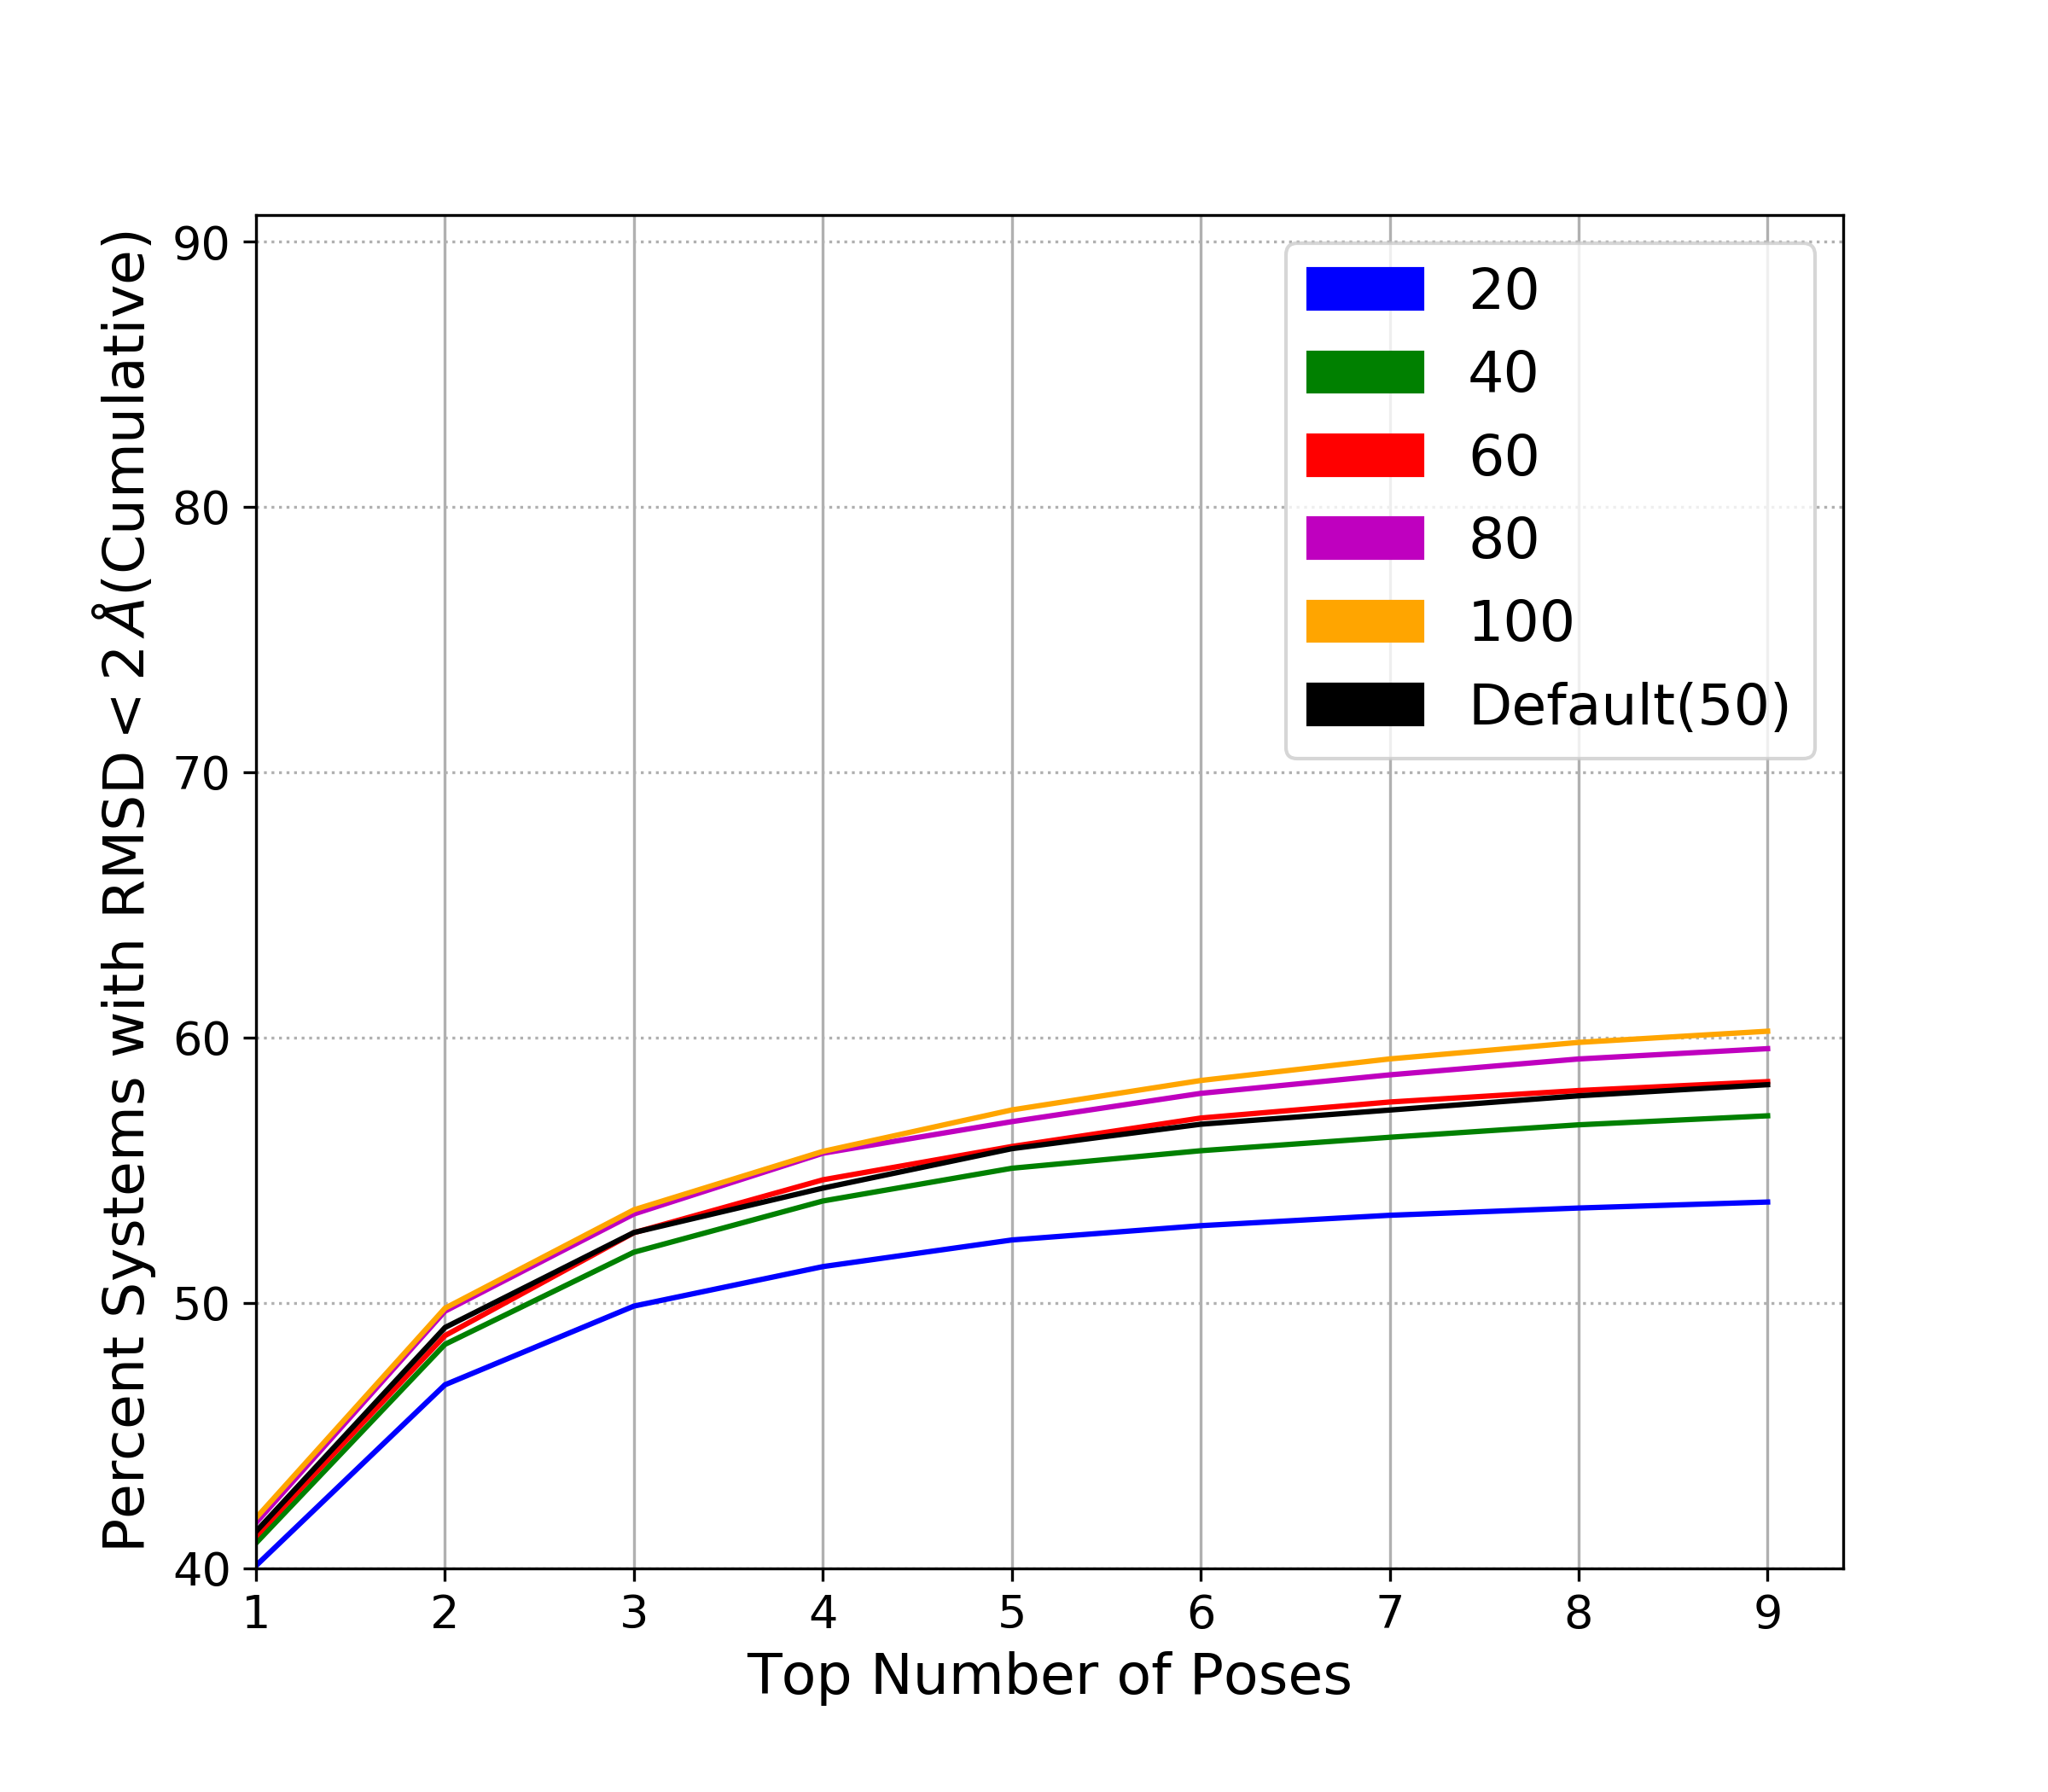
\includegraphics[width=\textwidth]{figures/crossdocking/sweep_mcsaved_line.png}
		\caption{Crossdocking}
		\label{fig:mcsaved cd}
        \end{subfigure}    
	\caption{}
	\label{fig:mcsaved}
\end{figure}    

Increases in the number of monte carlo saved increases the chances of sampling accurate docking poses. However, increases in the number of monte carlo saved will increase computational time, due to more poses needed to be sampled from each monte carlo chain and refinement required for a greater number of ligand conformations. As the number of monte carlo saved gets closer to 100, we see that the performance boost is reduced. Therefore, we select a value of 50 for the number of monte carlo saved to minimize the computational overhead while still increasing the performance of the docking routine.  

\begin{figure}    
        \begin{subfigure}[b]{0.48\textwidth}    
		\centering
		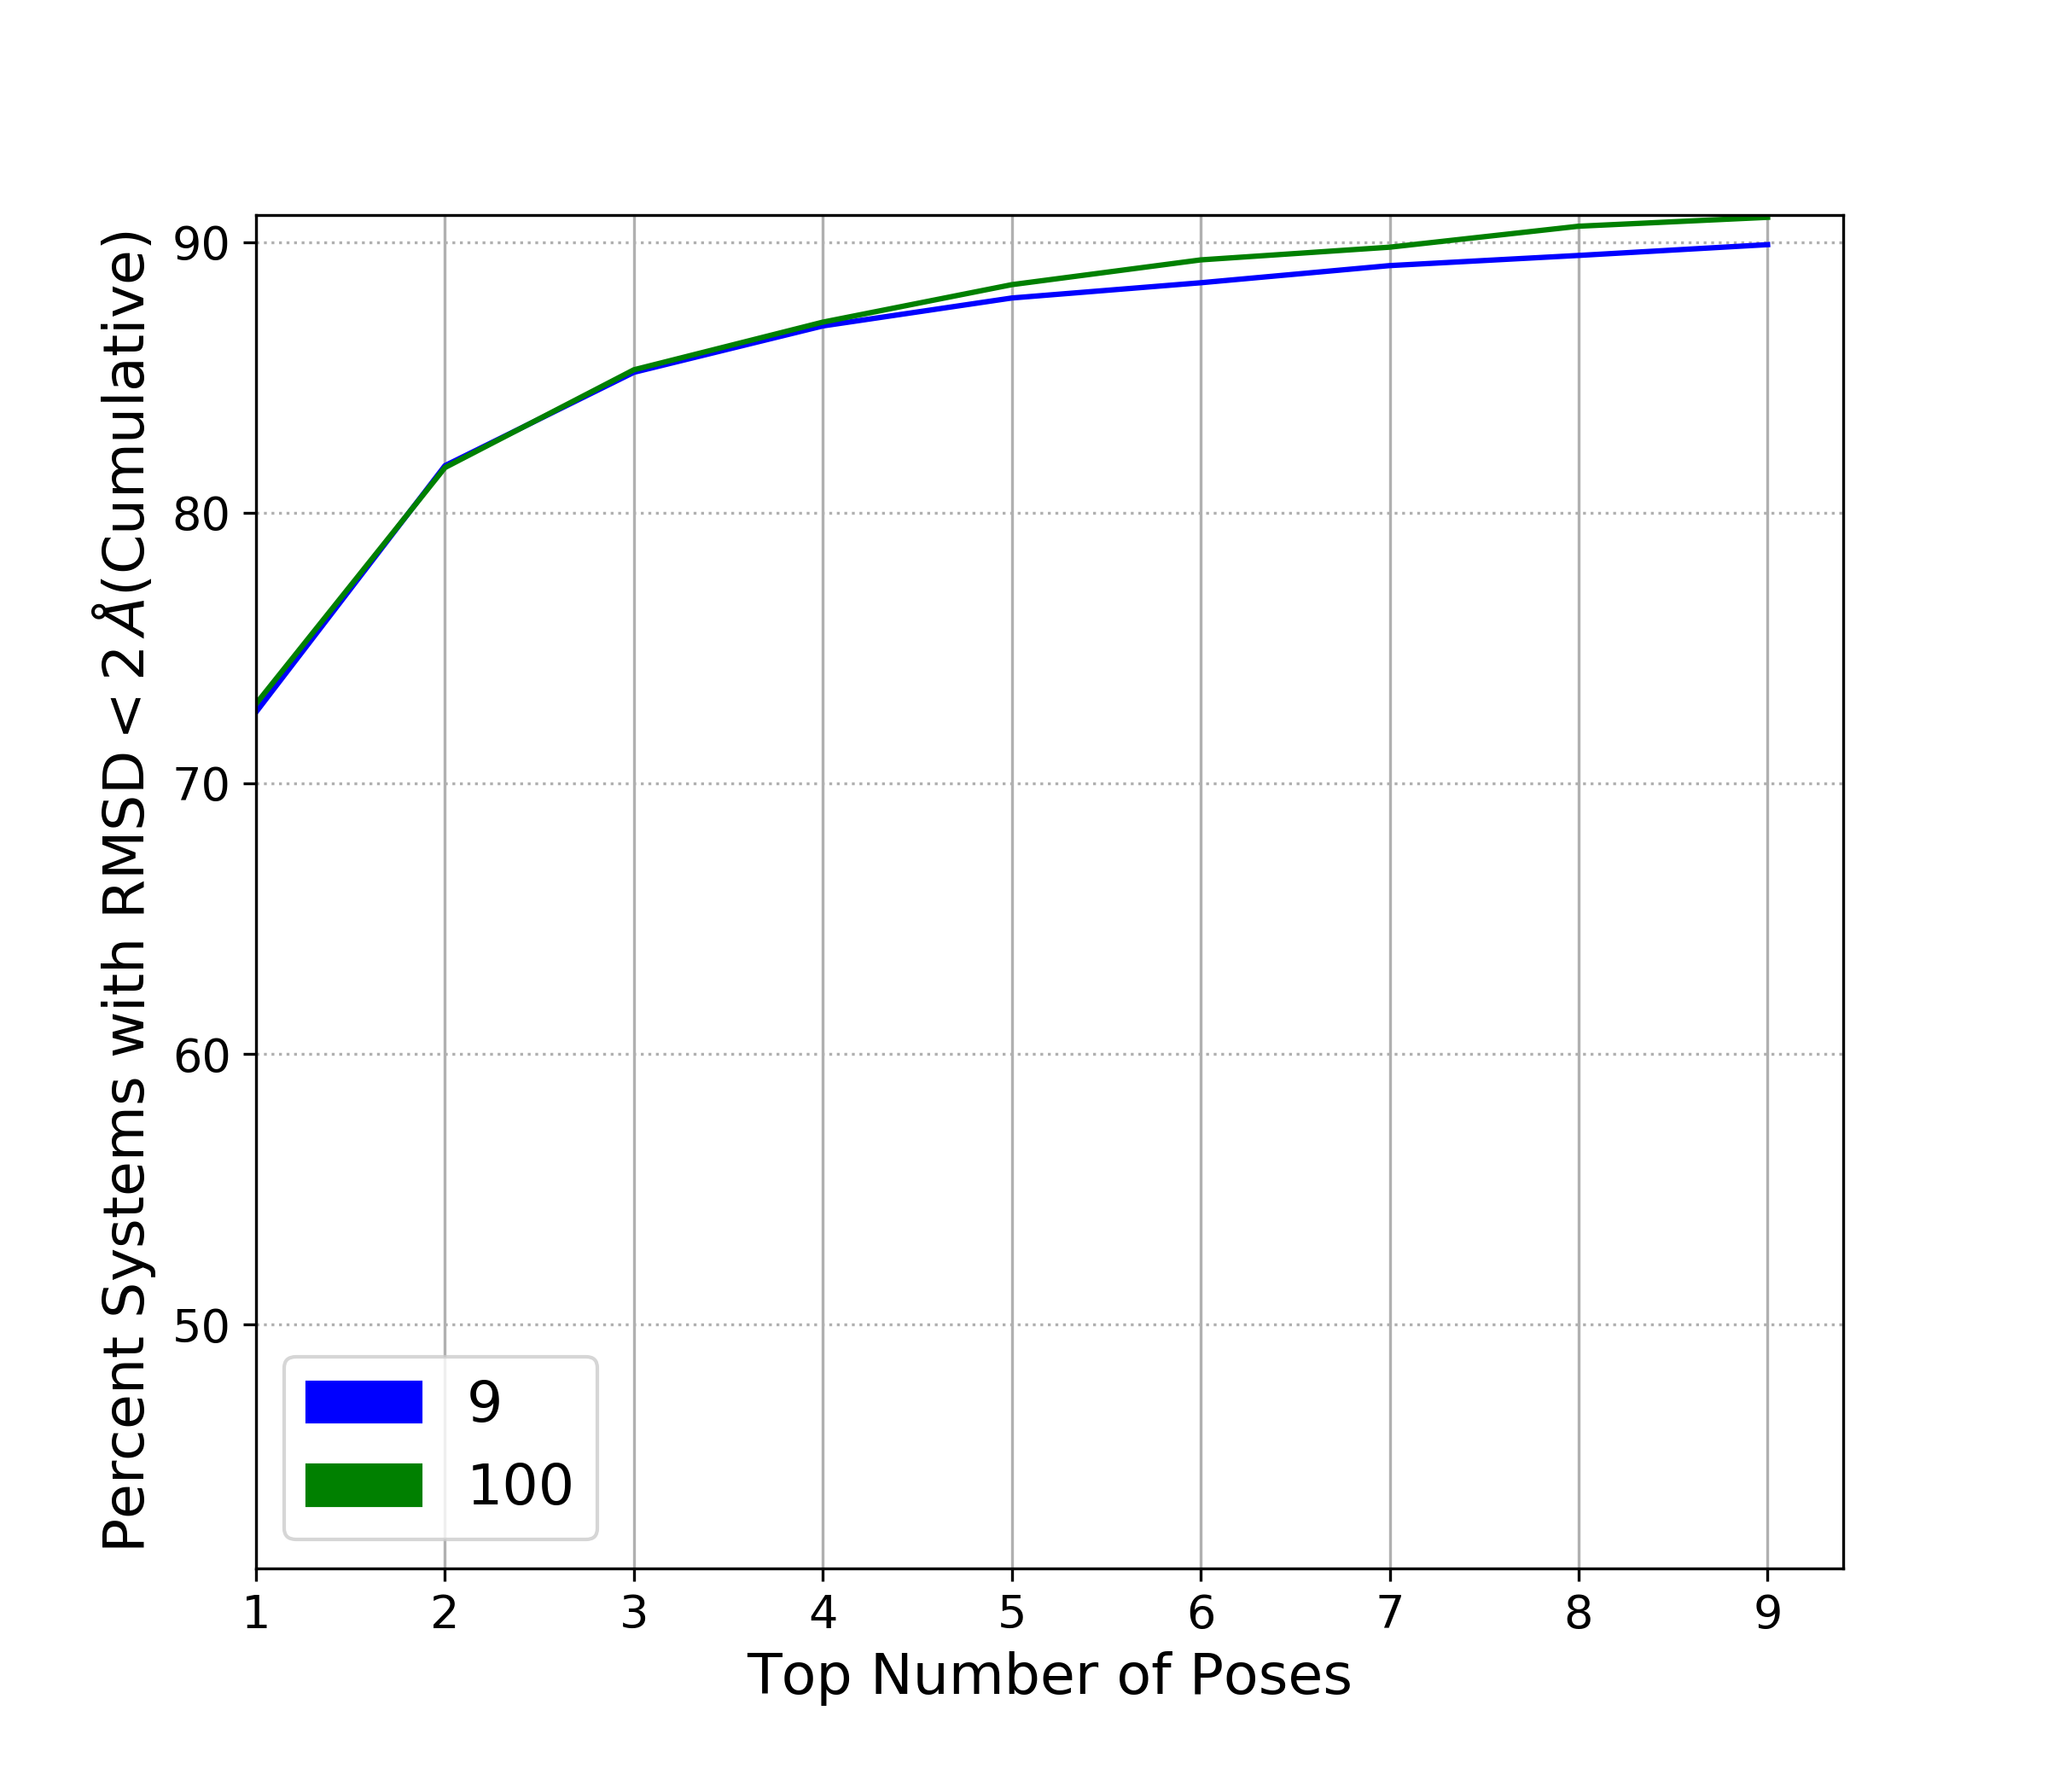
\includegraphics[width=\textwidth]{figures/redocking/sweep_num_modes_line.png}
		\caption{Redocking}
		\label{fig:num modes rd}
        \end{subfigure}    
        \begin{subfigure}[b]{0.48\textwidth}    
		\centering
		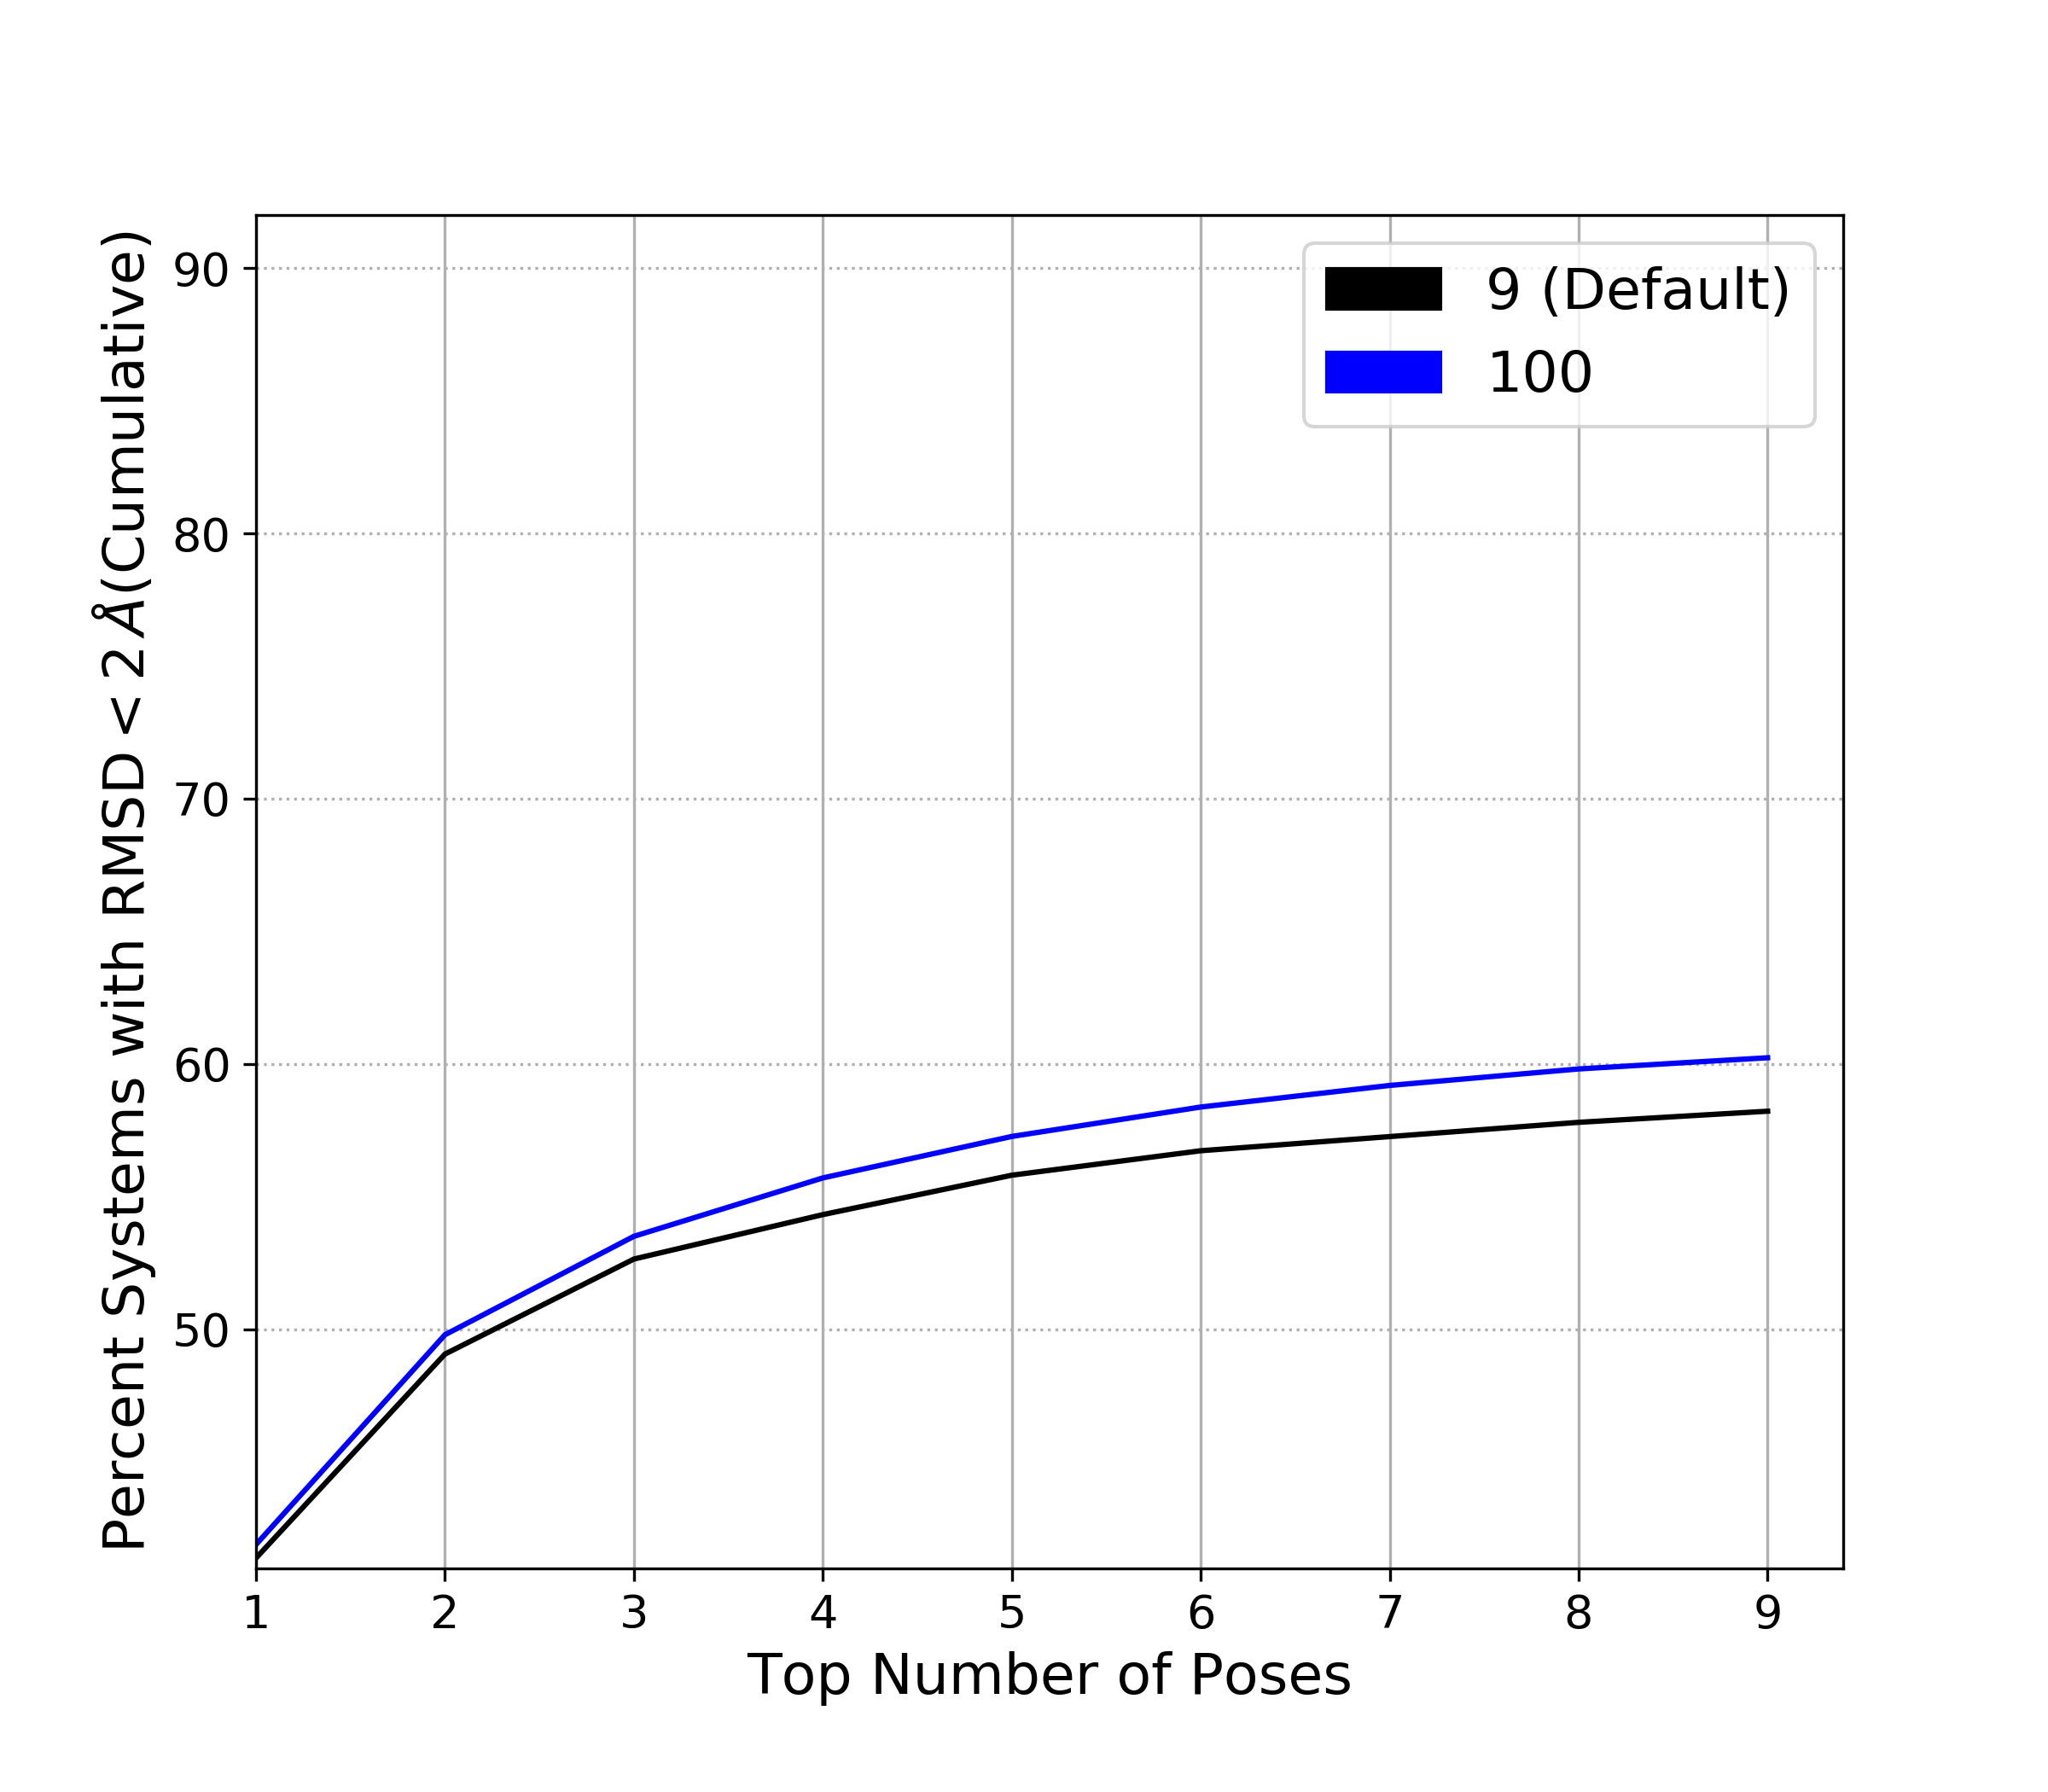
\includegraphics[width=\textwidth]{figures/crossdocking/sweep_num_modes_line.png}
		\caption{Crossdocking}
		\label{fig:num modes cd}
        \end{subfigure}    
	\caption{}
	\label{fig:num modes}
\end{figure}    

When looking at the first 10 poses, we see a marked increase in the performance of the docking routine with a large value for the number of modes. Since the molecular docking procedure is a sampling problem, with increased output conformations there is an increased liekelihood of finding the correct answer. We know that the CNNs rank the refined poses more accurately than the typical Vina scoring function, so if the docking procedure samples an accurate pose that Vina does not believe is high scoring the CNN will be able to rerank it to within the top 10.

\subsection{Gnina Performance}

\section{Discussion}



\begin{acknowledgement}

Please use ``The authors thank \ldots'' rather than ``The
authors would like to thank \ldots''.



\end{acknowledgement}

%%%%%%%%%%%%%%%%%%%%%%%%%%%%%%%%%%%%%%%%%%%%%%%%%%%%%%%%%%%%%%%%%%%%%
%% The same is true for Supporting Information, which should use the
%% suppinfo environment.
%%%%%%%%%%%%%%%%%%%%%%%%%%%%%%%%%%%%%%%%%%%%%%%%%%%%%%%%%%%%%%%%%%%%%
\begin{suppinfo}



\end{suppinfo}

%%%%%%%%%%%%%%%%%%%%%%%%%%%%%%%%%%%%%%%%%%%%%%%%%%%%%%%%%%%%%%%%%%%%%
%% The appropriate \bibliography command should be placed here.
%% Notice that the class file automatically sets \bibliographystyle
%% and also names the section correctly.
%%%%%%%%%%%%%%%%%%%%%%%%%%%%%%%%%%%%%%%%%%%%%%%%%%%%%%%%%%%%%%%%%%%%%
\bibliography{references}

\end{document}
